%\documentclass{cumcmthesis}
\documentclass[withoutpreface,bwprint]{cumcmthesis} %去掉封面与编号页
%\usepackage{graphicx}
%\usepackage{subfigure}
\usepackage{tabularx}
\usepackage{yhmath}
\usepackage{ctex}
\usepackage{appendix}
\usepackage{cite}
\title{基于动态解析几何和的UAV纯方位无源定位调整算法模型}
\tihao{B}            % 题号
\baominghao{202217241200}    % 报名号
\schoolname{华中科技大学}
\membera{卢凯}
\memberb{陈铭锐}
\memberc{房怿宽}
\supervisor{胡勇}
\yearinput{2022}     % 年
\monthinput{09}      % 月
\dayinput{15}        % 日
\usepackage{algpseudocode}
\usepackage{amsmath}

\makeatletter
\newif\if@restonecol
\makeatother
\let\algorithm\relax
\let\endalgorithm\relax
\usepackage[linesnumbered,ruled,vlined]{algorithm2e}%[ruled,vlined]{
\DeclareSymbolFont{yhlargesymbols}{OMX}{yhex}{m}{n}
\DeclareSymbolFont{ugmL}{OMX}{mdugm}{m}{n}
\DeclareMathAccent{\wideparen}{\mathord}{yhlargesymbols}{"F3}
\renewcommand{\algorithmicrequire}{\textbf{Input:}}  % Use Input in the format of Algorithm
\renewcommand{\algorithmicensure}{\textbf{Output:}} % Use Output in the format of Algorithm
\begin{document}
	\maketitle
\begin{abstract}
	\par 本文对于无人机集群无源方向定位系统进行研究。首先我们确定本题的解题目标为设计计算方法使集群中的无人机能够组成特定形状的编组,以及被动接收信号无人机基于\textbf{解析几何}和\textbf{迭代调整}的定位模型。在此思路下,遵循第一问中(1)、(2)、(3)小问的顺序,我们采用\textbf{平面空间可行域分割}的方法对于问题的本质进行探索,并辅以合适的计算机编程手段验证并优化无人机的定位及调整算法。
	\par 对于问题一(1):本题为双无偏圆弧-圆心无人机对第三者的定位问题,故此问题可抽象为平面几何求解问题。我们使用平面几何定理和简约的数学表达式给出了解析方程,并可以通过求解器求出数值解。
	\par 对于问题一(2):本题的数学模型也是一个双无偏圆弧-圆心无人机对第三者的定位问题。此时发射信号的无人机标签未知,在得到两个夹角后需要对发射无人机的标签进行猜测。此时第二问的问题集中在如何对于匿名无人机进行标签推断。为了进一步探索问题的实质,我们使用\textbf{可行域分割}的方法使用计算机模拟手段研究不同组态下解轨迹的运动问题。进而\textbf{对题目中“微小偏差”做了数学定义},并确立了我们设计的方法的唯一解条件。确定发射无人机编号后,本问题即化归为(1)的问题。
	\par 对于问题一(3):本题的情形下,发射信号无人机标签已知,其本身可能有偏。我们将本题的数学模型总结为有偏信号发射源下定位与规划问题。对一个与理想圆形编队略有随机偏差的无人机编队,基于\textbf{蒙特卡洛方法}发现采用编号FY00和\textbf{圆上3架最大间隔无人机}发射信号能大幅减小定位误差,从而确定了发射信号无人机的数目与选择方式。同时,我们设计了被接收信号无人机\textbf{“定位-位移”迭代调整算法},\textbf{仅5次迭代}使得编队收敛到较为理想圆形编队,\textbf{极径与极角相对误差均为$10^{-5}$数量级}。在生成随机误差数据以验证算法的鲁棒性时,我们使用蒙特卡洛法\cite{meta}对于可能产生的误差进行随机取样,使用程序模拟的方法提出了多信号源的精确定位算法。并由此提出\textbf{平均圆规划与调整算法}。
	\par 对于问题二:本题的情形下是一个非圆阵列定位与规划问题,针对锥形无人机编队,采用\textbf{分而治之}的思路,将问题转化为多个相关圆形编队调整策略,将无人机编队分为顶点无人机和非顶点无人机,结合\textbf{问题一(3)}中的方法,提出一个(3+1)\textbf{四阶段锥形无人机编队调整方案},经仿真通过调整可以将编队相邻无人机间隔标准差调整为初始情况的$0.5\%$左右。
	
	
	\keywords{\quad 几何动态解析\quad 可行域分割 \quad 蒙特卡罗方法 \quad 多阶段调整方案\quad 误差分析}
	
\end{abstract}
%\tableofcontents
	
	
%----------- 正文 ----------
%----------- 一、问题重述 ----------
		\section{问题重述}
		\subsection{问题背景}
		\par 无人机是“无人驾驶空中飞行器”(UAV)的简称。1917年首先由英国研制出来最先承担起军事功能,诸如目标定位跟踪技术在航空、航天和航海领域都有十分重要的地位。无源定位技术是指被动工作方式的目标定位技术,利用未知目标的辐射源信号进行定位和导航。相关的定位方法有通过相关时延参数的Fisher信息矩阵(FIM)法\cite{9020301}、深度学习方法\cite{9615429}等许多方法。
		\subsection{待求解的问题}
		\par 
		\begin{enumerate}
			\item{\textbf{问题一(1)}:}在已知三架编号已知、位置无偏差的无人机且其中一架为位于圆心的无人机FY$ 00 $为承担发射信号任务的无人机的既定条件下,根据圆周上其他的位置存在偏差的无人机被动接受的方向信号建立模型来完成对该被动接收信号无人机的纯方位无源定位。
			\item{\textbf{问题一(2)}:}在编队方式仍为圆周,且无人机数目仍为10架的相同条件下,修改发射信号的无人机为编号FY$ 00 $和FY$ 01 $的无人机与待定数量未知编号的无人机。发射信号的无人机的位置没有偏差,确定除了已知编号的无人机FY$ 00 $和无人机FY$ 01 $外,最少需要几架未知编号的无人机作为位置无偏差的无人机来发射信号以期望实现无人机的有效定位。
			\item{\textbf{问题一(3)}:}在编队方式与无人机数目基础条件均不变的基础上,设定无人机所处圆周的半径为100m。初始时刻无人机的位置确定但略有偏差,试确定在编号为FY$ 00 $的无人机和圆周上数量不超过三架的无人机作为发射信号的无人机的条件下,忽略每次调整的时间,调整到理想位置使九架无人机均匀的分布在某个圆周上的最优调整方案。
			\item{\textbf{问题二}:}
			在问题四中,无人机编队方式变化为锥形,相邻两架无人机间距相等,具有良好的几何性质。待求解问题有如下:
			\begin{itemize}
				\item 对编队中的任意一架无人机,若以无人机间距为半径,另外某架无人机为圆心,一定可以找到这样的圆使该无人机位于圆上,从而将定位问题转化为问题一的情景;
				\item 对编队中任意一架无人机,上述圆至少可以找到两个,仅有两个这样的圆的情况是该飞机位于锥形顶点的时候(FY01,FY11,FY15)。基于顶点的特殊性,我们将调整方案分为两个子方案:调整非顶点飞机方案与调整顶点飞机方案;
			\end{itemize}
			基于上述分析,我们设计一个两阶段的调整方案,对无人机编队中各机位置进行调整,使最终所得编队中相邻飞机的间距相等,通过模拟仿真证明我们算命的有效性。
		\end{enumerate}
%----------- 二、问题分析 ----------
	\section{问题分析}
		\subsection{问题一(1):}
		在第一题的大背景下,我们可以知道,无人机的数目和编队的方式,并且给定的条件为有三架已知编号且位置没有误差的无人机作为发射信号的无人机。我们需要根据其余位置有偏差的无人机被动接受到的方位信号即三个角度信息从而实现定位。
		\subsection{问题一(2):}
		在问题一(2)中,我们首先假设对于任意的$D_i$,通过测量$D_0,D_1,D_j$三个无人机的位置,得到两个小角$\alpha_1,\alpha_2$,进而能够确定自己在$D_0 - D_1$坐标系中的位置。
		
		可以假定的是,对于任意的$D_i$,在接收其他无人机的发射信号时,有以下公共知识:
		\begin{itemize}
			\item	位置待定无人机自身的编号$i$,
			\item	可以辨识从$D_0$与$D_1$发出的信号,但不确定第三个信号来源,
			\item	无人机机群的结构,即各个编号无人机在圆上的大致位置与顺序,任意两个无人机不能交换顺序。
			\item 	待定无人机相对于理想位置的偏差较小,即$ {\lVert \omega_i \rVert}^2 < r_0 $.
		\end{itemize}
		\begin{figure}[htb]
			\centering
			\subfloat[组态1]{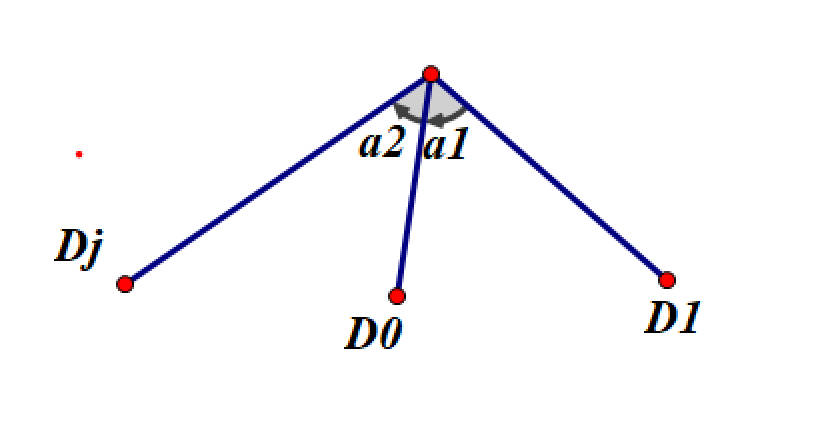
\includegraphics[width=0.4\linewidth]{../figures/1}}
			\subfloat[组态2]{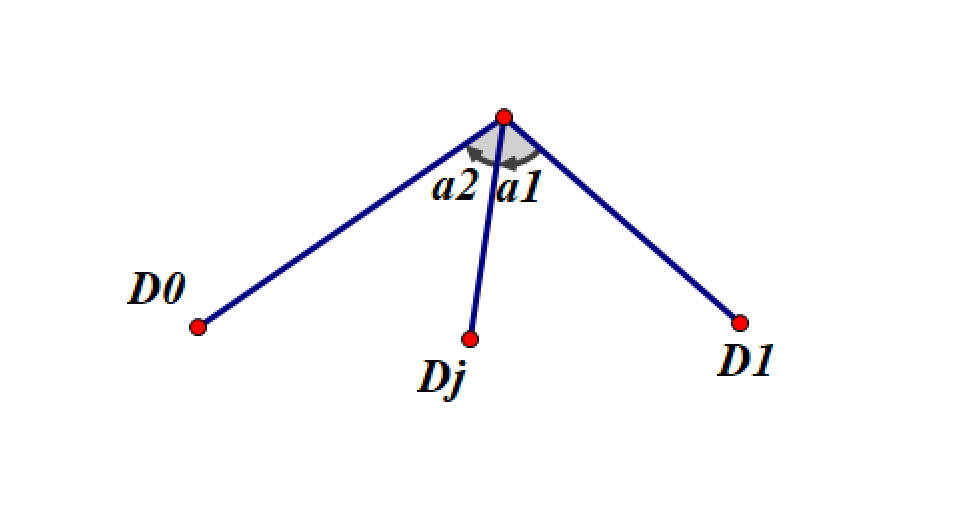
\includegraphics[width=0.4\linewidth]{../figures/2}}
			\caption{可能出现的两种组态}
			\label{fig1}
		\end{figure}
		基于以上公共知识,需要设计算法$D_i = f(\alpha_1, \alpha_2)$求解$D_i$在$D_0 - D_1$坐标系中的位置。
		\subsection{问题一(3):}
		在问题三中,我们认为9架飞机均匀分布在以编号FY00为圆心的情况为理想分布,要求在各无人机所在位置与理想位置略有偏差的初始情况下,每次通过选取FY00和圆上最多三架飞机发射信号,其余飞机根据接收到的方向信息调整位置。我们得到如下分析和和假设:
		\begin{itemize}
			\item	每个飞机知道自身的编号$i$和自身的理想分布位置$(x_{ideal},y_{ideal})$
			\item   飞机对每个接收到的信号,能够识别其信号来源无人机的编号$i$,
			\item	每个飞机根据接收到的方向信息进行定位,得到估计定位$(\hat{x},\hat{y})$,通过位移一段距离进行调整位置调整,位移在直角坐标系下表示为$(\Delta{}x,\Delta{}y)$,可以度量估计定位$(\hat{x},\hat{y})$和理想位置$(x_ideal,y_ideal)$的偏差来确定,
			\item	由于发射信号的飞机可能有误差,所以使用基于问题一的定位方法会产生误差,
			\item 	待定无人机相对于理想位置的偏差较小,即$ {\lVert \omega_i \rVert}^2 < r_0 $.
		\end{itemize}
		基于上述分析,我们建立了一个位置调整算法,对输入的起始情况,对编号为$i$的飞机,通过多次迭代$(\Delta{}x,\Delta{}y)_i$调整位置,将机群调整到理想分布上。该算法可以分为选取发射信号飞机、接收信号与定位、位置调整三个部分。
		\subsection{问题二:}
		 在问题二中,无人机编队为锥形,相邻两架无人机间距相等,具有良好的几何性质。我们对问题有如下分析:
		\begin{itemize}
			\item 对编队中的任意一架无人机,若以无人机间距为半径,另外某架无人机为圆心,一定可以找到这样的圆使该无人机位于圆上,从而将该定位问题转化为问题一的情景;
			\item 对编队中任意一架无人机,上述圆至少可以找到两个,仅有两个这样的圆的情况是该飞机位于锥形顶点的时候(FY01,FY11,FY15)。基于顶点的特殊性,我们将调整方案分为两个子方案:调整非顶点飞机方案与调整顶点飞机方案;
		\end{itemize}
		基于上述分析,我们设计一个两阶段的调整方案,对无人机编队中各机位置进行调整,使最终所得编队中相邻飞机的间距相等,通过模拟仿真证明我们算命的有效性。
%----------- 三、模型的假设与约定 ----------
	\section{模型的假设与约定}
		\begin{itemize}
			\item{} 无人机机群的结构即各个编号无人机在圆上的大致位置与顺序,任意两个无人机不能交换顺序。
			\item{} 考虑电磁信号的损耗和中断等不良情况,我们假定待定无人机相对于理想位置的偏差较小,且收到的电磁信号清晰可辨。
			\item{} 在一定范围内,不同无人机发射信号不会产生杂糅或者耦合的情况。
			
		\end{itemize}
%----------- 四、符号说明及名词定义 ----------
	\section{符号说明及名词定义}
		\begin{center}
			\begin{table}[H]
				\caption{本论文所使用的符号}
				\begin{tabularx}{\textwidth}{p{0.08\textwidth}X}
					\toprule	
					$D_i$ & 编号为$i$的无人机的理想位置  \\
					$\widehat{D_i}$ & 编号为$i$的无人机的有偏实际位置  \\
					$D_i(\rho,\theta)$ & 用极坐标表示的无人机的位置 \\
					  
					$\overrightarrow{D_iD_k}$ & 从$D_i$指向$D_k$的矢量 \\
					$\omega_i$      & 编号为$i$的无人机的误差矢量,即$\overrightarrow{\widehat{D_i}D_i}$ \\
					$\bigodot O_i$    & 第$i$个理想圆  \\
					$ \alpha_i $	&两架无人机发射信号与接受信号无人机之间的夹角\\
					$ \beta_i $	    &发射信号无人机在极坐标系下的极角\\
					$ \omega$ 		&衡量估计无人机位置的偏差值\\
					$ \eta $		&对估计位置信息进行修正的学习率\\
					\bottomrule
				\end{tabularx}
			\end{table}

		\end{center}
%----------- 五、模型的建立与求解 ----------
	\section{模型的建立与求解}
		\subsection{问题一(1)}
			\subsubsection{问题一(1)模型的建立}
			\par 问题一首先限定了编队的飞机数目为10架并且编队方式为圆形编队,且要求其中一架无人机(编号为FY$ 00 $)位于圆心,而其余九架无人机位于相应的圆周上面。值得注意的是,无人机会基于自身感知的高度信息,均保持在同一个高度上飞行,因此我们可以将问题的求解模型确定在一个高度平面来方便求解下列各个问题。
			\par 
			而第一题的第一问则进一步明确无人机的角色:位于圆心的无人机(FY$ 00 $)和编队中另 $ 2 $ 架无人机发射信号,而其他无人机则是被动接受该三架无人机发射信号的角色。同时一个重要的条件是:模型要求在发射信号的无人机位置无偏差且编号已知的情况下完成其他被动接受信号的无人的定位。基于上述已知设定信息,我们可以首先将定位问题转换为二维平面上的位置求解问题。因为圆周的位置具有\textbf{高度对称性},因此不妨假设其中两台圆周上已知编号的信号发射无人机其中一台的编号为FY$ 01 $.因此我们可以在二维平面上选取编号为FY$ 00 $的无人机为原点,编号为FY$ 01 $的无人机为$ X $轴正方向的一点,从而建立笛卡尔右手坐标系如下图\ref{1-1}。
			\begin{figure}[htb]
				\centering
				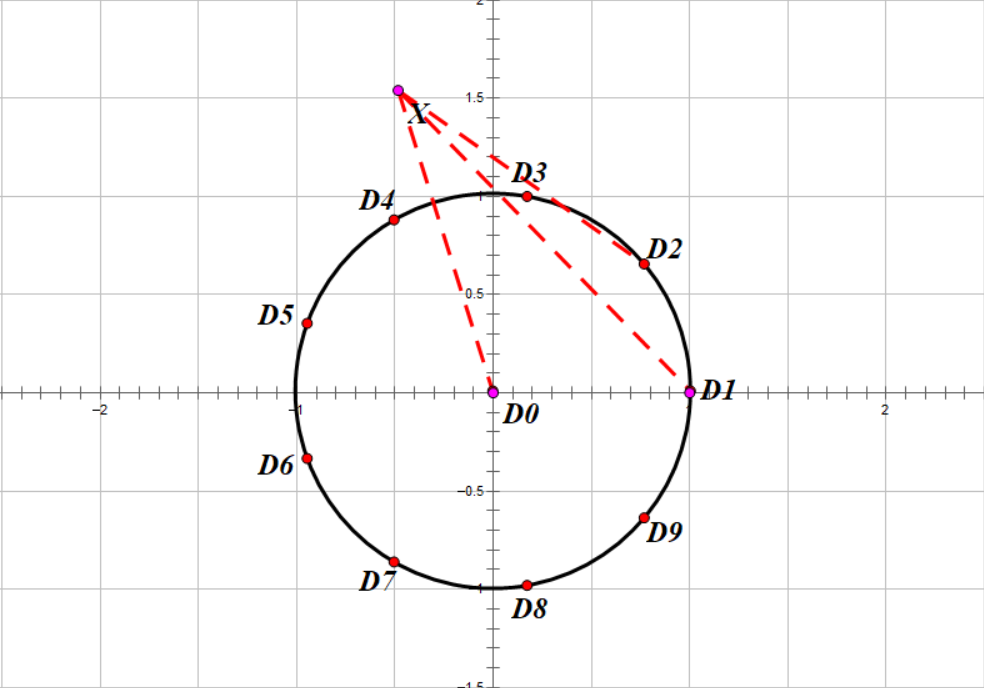
\includegraphics[width=0.7\linewidth]{./figures/Question1-1.png}
				\caption{问题一:定位模型坐标系}
				\label{1-1}
			\end{figure}
			在已知三架编号已知且位置无偏差的无人机后,我们可以在该坐标系中按直角坐标。同时对于编队中其他待定位的无人机,我们都可以得到与三架发射信号无人机的方位信息:任意两架发射信号无人机与待定位无人机的夹角。夹角代表着方向向量直接的位置关系,故应在表示待定位无人机的直角坐标后确定发射信号的无人机与待定位无人机连线的方向向量,进而再表示出夹角然后求解。
			\subsubsection{问题一(1)的具体求解}
			\par 基于第一问的定位模型,我们建立以已知编号FY$ 00 $ 的无人机为原点$ D_0 $ ,而另外两架已知编号的$ \text{无人机}i\text{与无人机}j $ $ \text{无人机}i\text{与无人机}j $ 分别设为$ D_i\text{与}D_j $ ,其极坐标对应的为$ \left( R,\beta _i \right) ,\left( R,\beta _j \right)  $ ,其中$ \beta _i\text{与}\beta _j $ 均可通过编号得到,为已知数据。不失一般性,我们将其他所有待定位的无人机$ D_X $ 的极坐标设为$ \left( \rho ,\theta \right)  $ 。根据题意我们可知无人机$  D_X $ 会接收到位于设定原点的无人机$ D_0 $ 和$ \text{无人机}D_i\text{与无人机}D_j $ 发射的电磁信号,进而可以提取的信号为:该无人机$ D_X $ 与任意两架发射信号的$ \text{无人机}D_i\text{与无人机}D_j $ 连线之间的夹角,即$ \left( \begin{array}{c} 	3\\ 	2\\ \end{array} \right)  $ 共三个角度的方位信息。根据几何知识,可以得到该三个角中最大的角为其余两个角的和。因此,为减少信息的冗余性,我们只利用其中两个角:$$ \alpha _i=\angle D_0 D_X D_i\text{,}\alpha _j=\angle D_0 D_X D_j $$ 
			\par 至此,我们从极坐标转至直角坐标系: 
			$$ D_0\text{:}\left( 0,0 \right)  $$ $$ D_i\text{:}\left( R\cos \beta _i,R\sin \beta _i \right)  $$ $$ D_j\text{:}\left( R\cos \beta _j,R\sin \beta _j \right)  $$ $$ D_X\text{:}\left( \rho \cos \theta ,\rho \sin \theta \right)  $$ 
			\par 因此可以进而得到三个向量:
			$$ \overrightarrow{D_0D_X}=\left( \rho \cos \theta ,\rho \sin \theta \right)  $$ $$ \overrightarrow{D_iD_X}=\left( \rho \cos \theta -r\cos \beta _i,\rho \sin \theta -R\sin \beta _i \right)  $$ $$ \overrightarrow{D_jD_X}=\left( \rho \cos \theta -R\cos \beta _j,\rho \sin \theta -R\sin \beta _j \right)  $$ 	
			\par 紧接着,我们通过三个向量分别利用余弦定理,分别表示出$ \alpha _i\text{与}\alpha _j $: 
			$$ \cos \alpha _k=\frac{\rho ^2\sin ^2\theta -R\rho \cos \beta _k\cos \theta +\rho ^2\cos ^2\theta -R\rho \sin \beta _k\sin \theta}{\rho ·\sqrt{\rho ^2\sin ^2\theta +r^2\sin ^2\beta _k-2R\rho \sin \beta _k\sin \theta +\rho ^2\cos ^2\theta +R^2\cos ^2\beta _k-2R\rho \cos \beta _k\cos \theta}}\\   $$ 
			
			$$\text{令} k=i,j\text{可分别得}\left\{ \begin{array}{l} 	\cos \alpha _i=\frac{\rho -R\cos \left( \theta -\beta _i \right)}{\sqrt{\rho ^2+R^2-2\rho R\cos \left( \theta -\beta _i \right)}}\\ 	\cos \alpha _j=\frac{\rho -R\cos \left( \theta -\beta _j \right)}{\sqrt{\rho ^2+R^2-2\rho R\cos \left( \theta -\beta _j \right)}} \end{array} \right.  $$ 
			\par 由此求解 两个方程:$ \text{通过}\frac{\rho}{R}\text{和}\theta \text{表示的}D_X\text{具体坐标} $ 从而完成定位。
			
		\subsection{问题一(2)}
			经过我们的研究,我们认为需要除了在圆心的0号,还需要在圆弧上的1号和另外一个j号共三架飞机发射信号才能确定任意一架飞机i的位置。
			我们的位置解算算法遵循机组组态分析、推断匿名第三者编号、可行域分割的步骤求出$D_i$的坐标。在使用逐步分割可行域的方式求解位置坐标时,我们针对多解的情况,着重讨论了对于“略有偏差”的数学定义。
			\subsubsection{算法的求解过程分析}
			对于问题$D_i = f(\alpha_1, \alpha_2)$,因为第一问中我们已经求解出了对于确定圆周上两个信号发射飞机的编号时,待测飞机位置的解析算法。本问我们首先需要确定第三架飞机是标签为几的飞机。以待测飞机为2号机,匿名第三信号发射机为3号机为例,建立数学几何模型并阐释我们的算法。
			\paragraph{机组组态分析}
			待测飞机为2号机的情况下,2号机接收到的三个角度值遵循$\angle D_jD_2D_1 =\angle D_jD_2D_0 + \angle D_jD_2D_1$,符合图\ref{fig1}中所示组态1的类型。
			\paragraph{匿名第三者位置分析}
			在组态1的情况下,匿名第三者编号$j=3,4,5,6$中的一个。
			\paragraph{可行域}
			对于所有可能的$D_j$,现已确定$\angle D_jD_2D_0 = \alpha_1$,$|D_jD_0|= r$,对于此类定弦定角问题,有优弧$\wideparen{D_jD_2D_0}$上的点为所有可能的$D_2$的位置。
			对于确定的$\angle D_0D_2D_1 = \alpha_2$,$|D_1D_0|= r$优弧$\wideparen{D_0D_2D_1}$上的所有点为所有可能的的$D_2$的位置。
			\begin{figure}[htb]
				\centering
				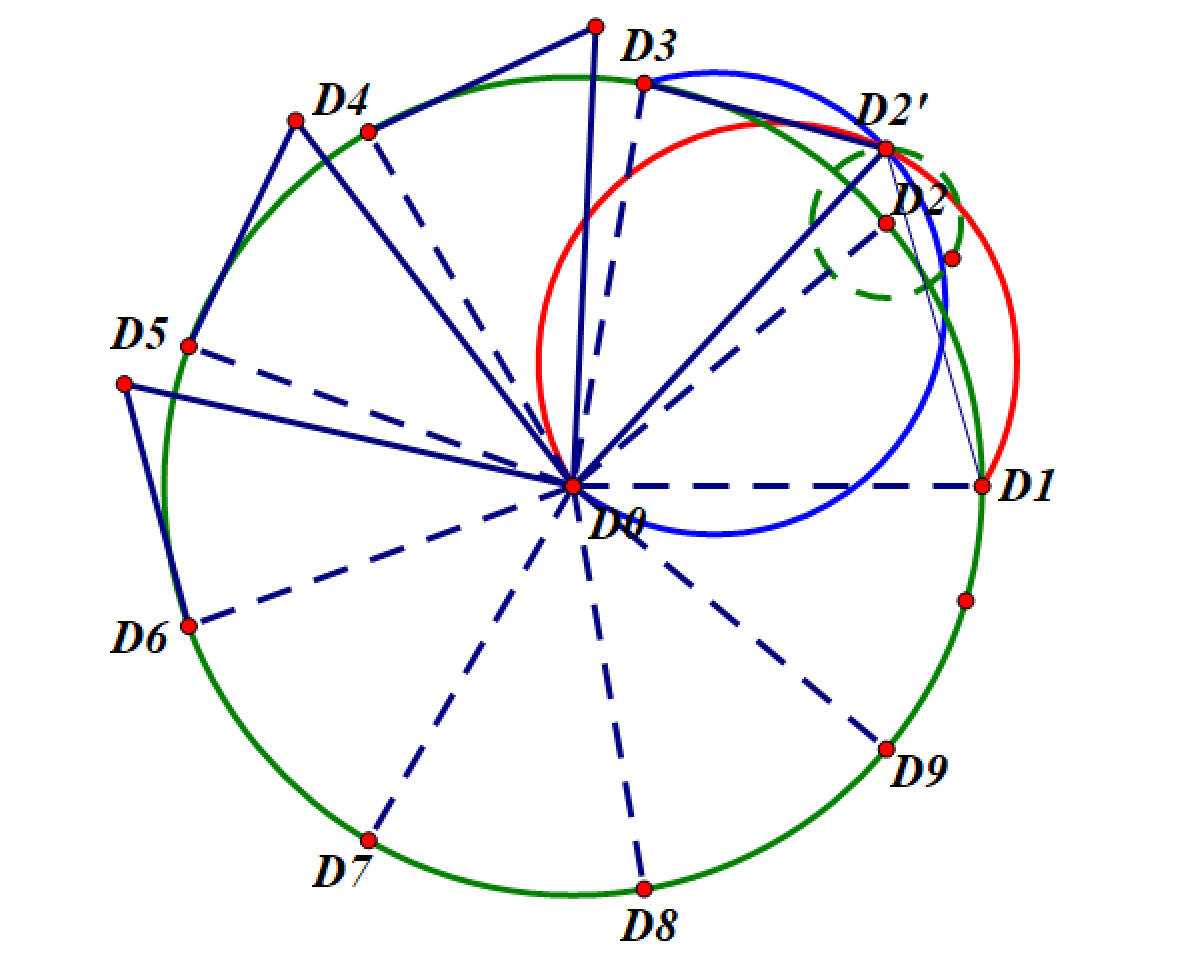
\includegraphics[width=0.4\linewidth]{./figures/3}
				\caption{$\angle D_3D_2D_0$ 的可行域$\wideparen{D_3D_2D_0}$与$\angle D_0D_2D_1$ 的可行域$\wideparen{D_0D_2D_1}$}
				\label{fig3}
			\end{figure}
		
		
			如图\ref{fig3}所示,对于有微小偏差的无人机$D_2'$,当假设匿名第三者为无人机3时,有可能位置$P$。同理,分别建立匿名第三者$j=4,5,6$时,$D_2'$的可能位置,分别标记为$Q,R,S$,如图\ref{fig4}.
			
			\begin{figure}[htb]
				\centering
				\subfloat[所有可能可行域集合]{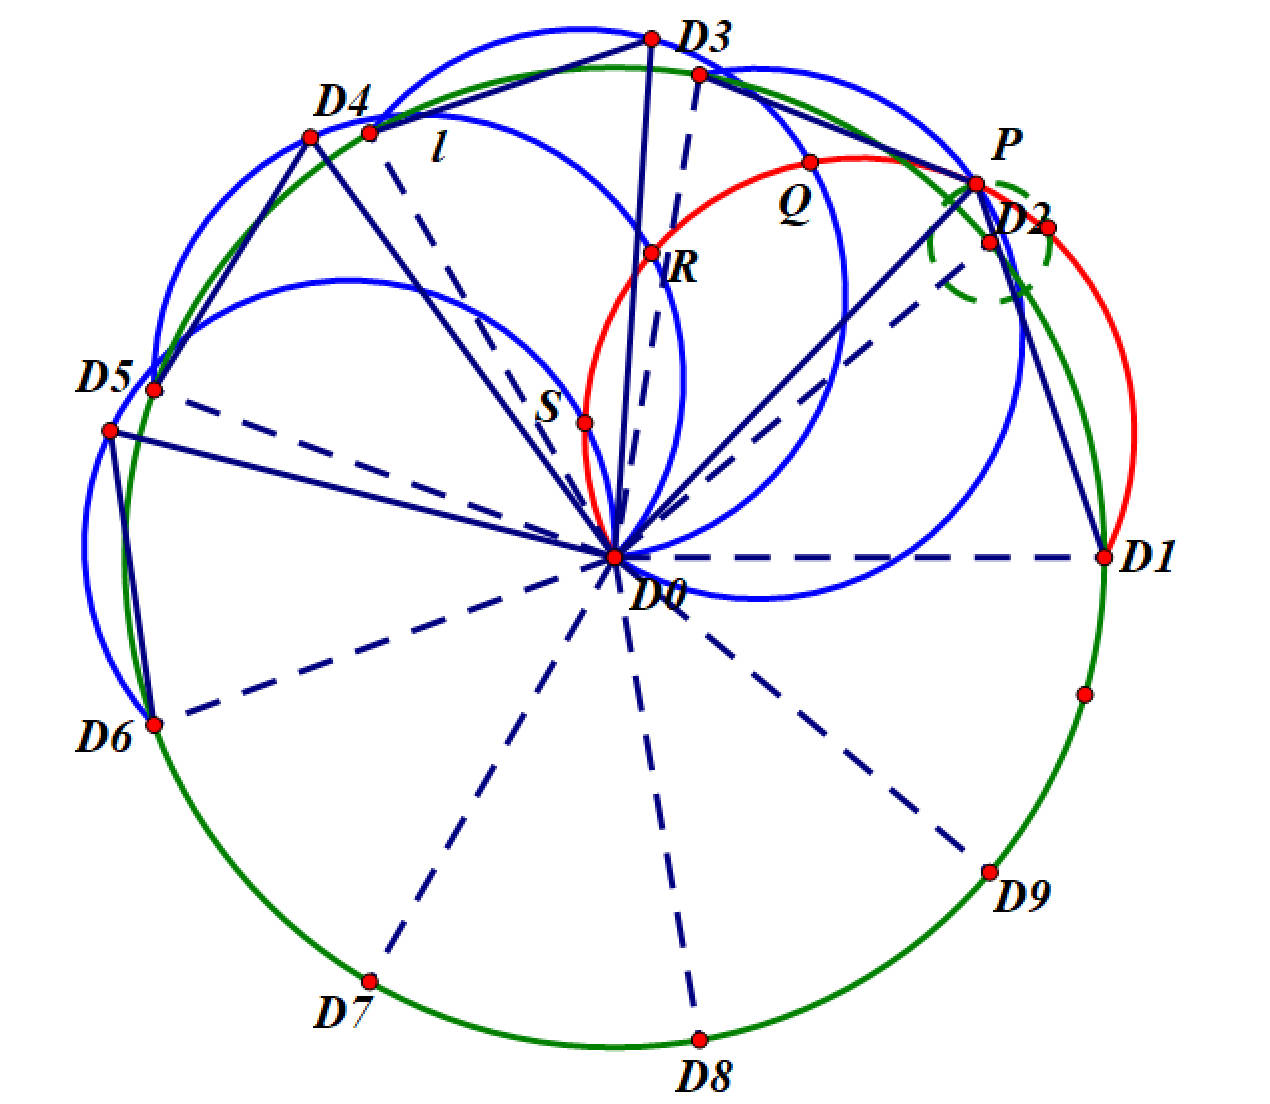
\includegraphics[width=0.3\linewidth]{../figures/4}}
				\subfloat[$D_2'$的可能位置$P,Q,R$]{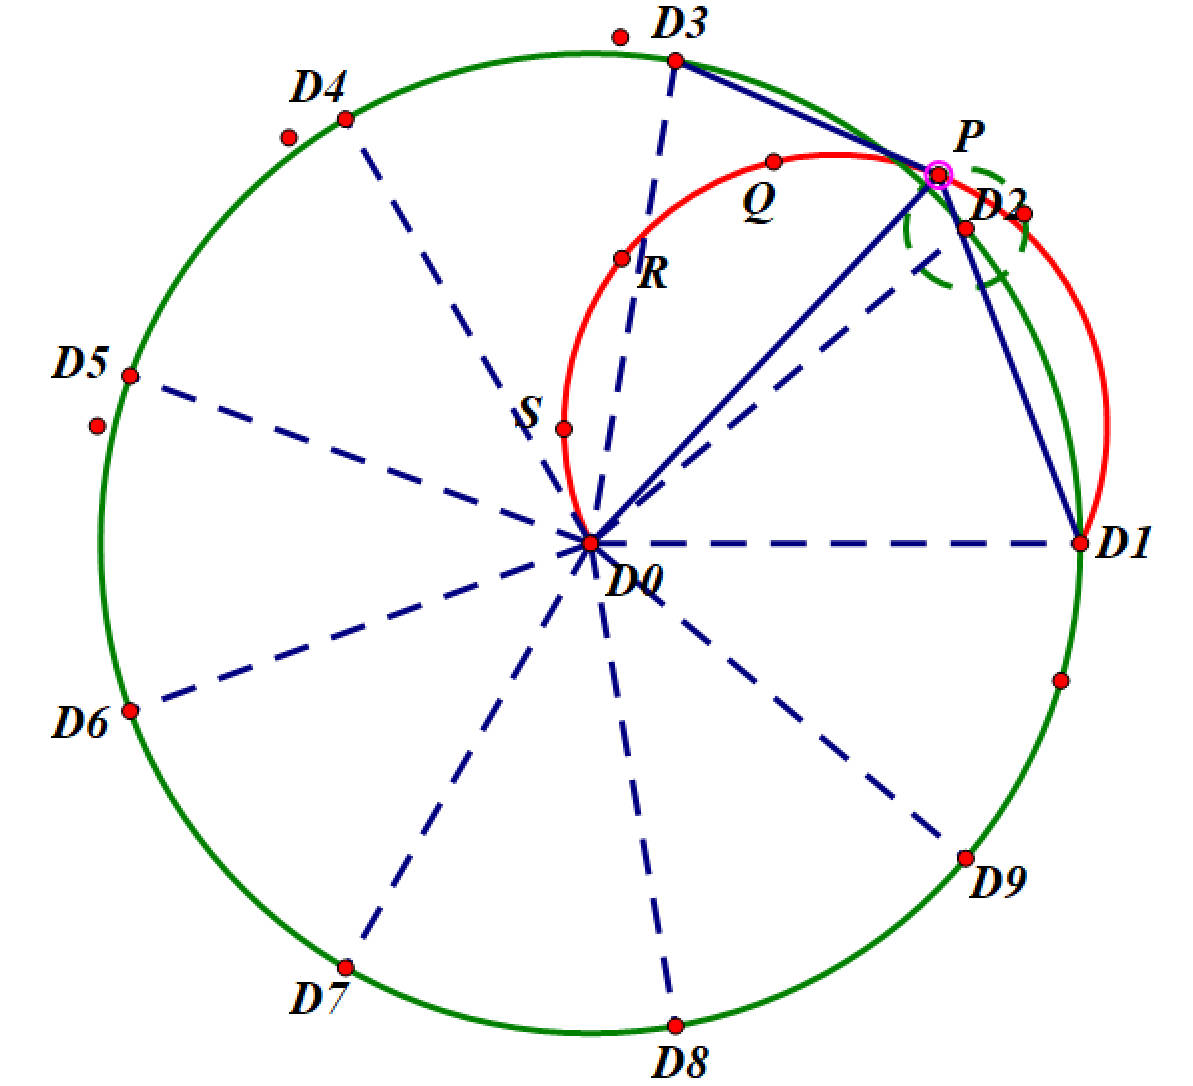
\includegraphics[width=0.3\linewidth]{../figures/5}}
				\caption{$D_2'$的可能位置的求解}
				\label{fig4}
			\end{figure}
			
			至此,对于不确定匿名第三者的情形,飞机$D_i$($D_2$)由于不能确定第三者编号产生了自己的位置猜测$P,Q,R,S$,在图\ref{fig4}的情形下,易确定$R,S$的情形不符合题设从而排除,然而我们观察到当2号机偏差很大时(即$\lVert\omega_i\rVert =\overrightarrow{D_2D_2'} $很大时)有可能出现情形如图\ref{fig6}.此时若认为第三者为4号机,则会有位置错误估计Q,而不是其实际位置P。因为此种情况的存在,我们就不能单纯地使用推断点距离理想点最近的一点作为测量结果,而要对“偏差较小”进行数学定义。
			\begin{figure}[htb]
				\centering
				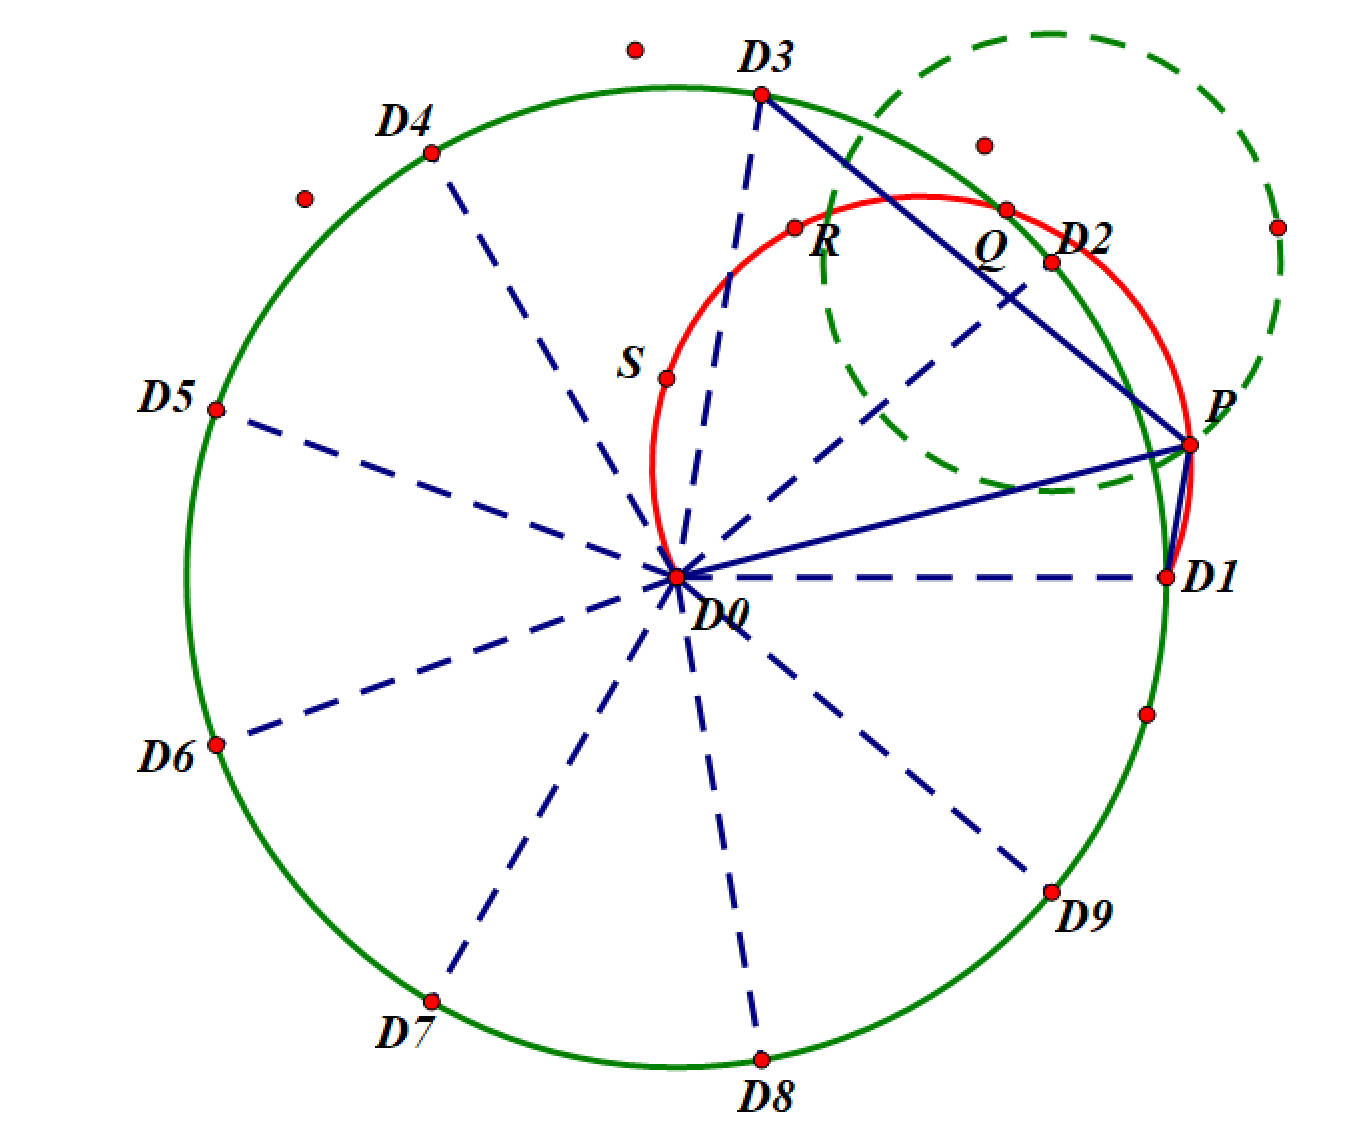
\includegraphics[width=0.3\linewidth]{./figures/6}
				\caption{偏差很大时的一种特殊情况}
				\label{fig6}
			\end{figure}
		
		
			\paragraph{多解分析}
			因为在三架飞机定位的模式下,匿名第三者未知。这种情况下待定位飞机对于自己的位置估计就可能出现多解的情况。然而我们发现,在待定位飞机距离无偏差位置很远的时候,不能通过解的合理性排除多解情况。为了保证我们能够使用推断点距离理想点最近的一点作为测量结果,我们进一步探索了多解的可排除情况的边界条件。
			
			
			当$ D_2' $ 运动在区域:$ \lVert \omega _2 \rVert \le r_0 $ 内时,$ \text{运动点}P\text{、}Q\text{、}R\text{、}S\text{的集合分别记为}\mathcal{P}\text{、}\mathcal{Q}\text{、}\mathcal{R}\text{、}\mathcal{S} $ 建立动态几何解析模型,使$ D_2' $在其运动区域边界上运动时,跟踪$P,Q,R,S$的轨迹,其内部即为$\mathcal{P}\text{、}\mathcal{Q}\text{、}\mathcal{R}\text{、}\mathcal{S}$.
			
			\begin{figure}[H]
				\centering
				\subfloat[$r_0$很小时的运动轨迹情况]{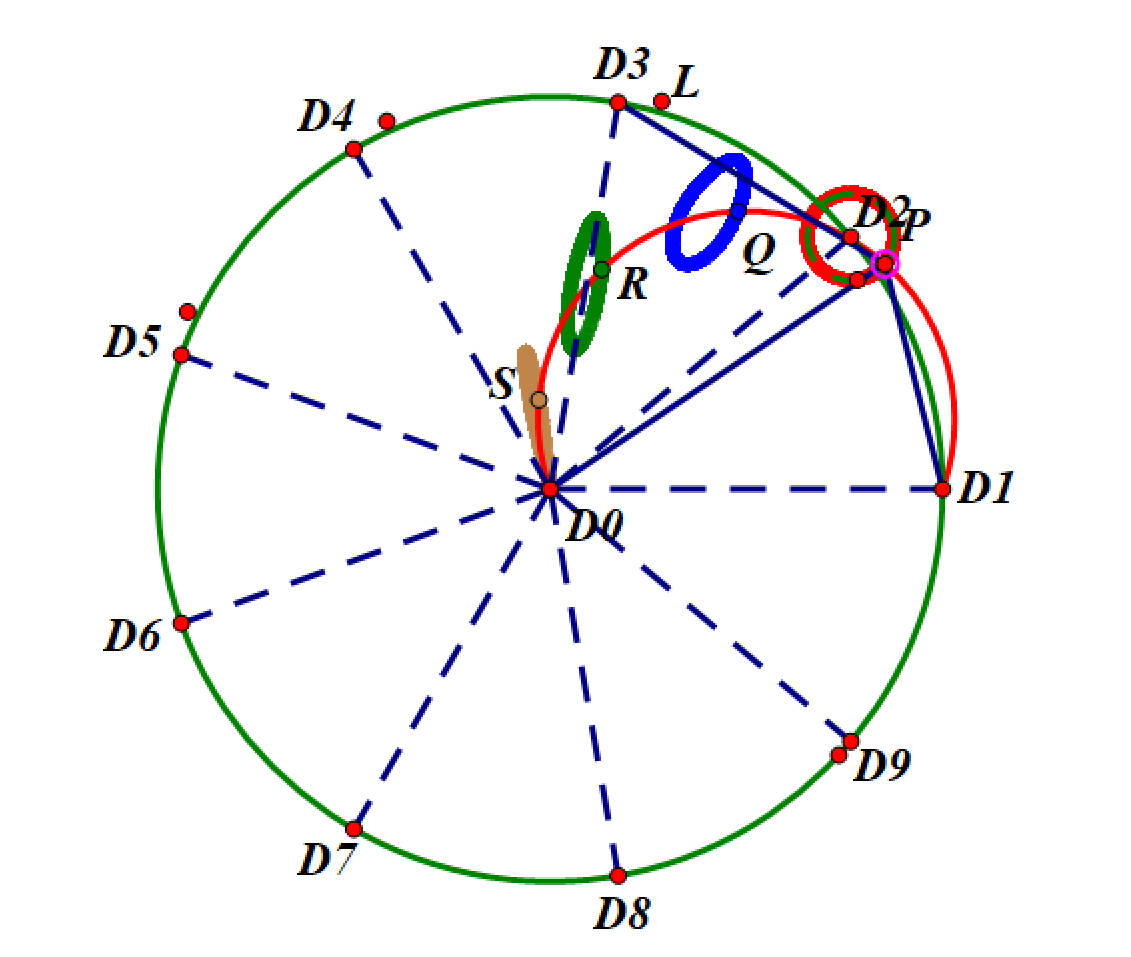
\includegraphics[width=0.23\linewidth]{../figures/7}}
				\subfloat[$r_0$处于临界时的运动轨迹情况]{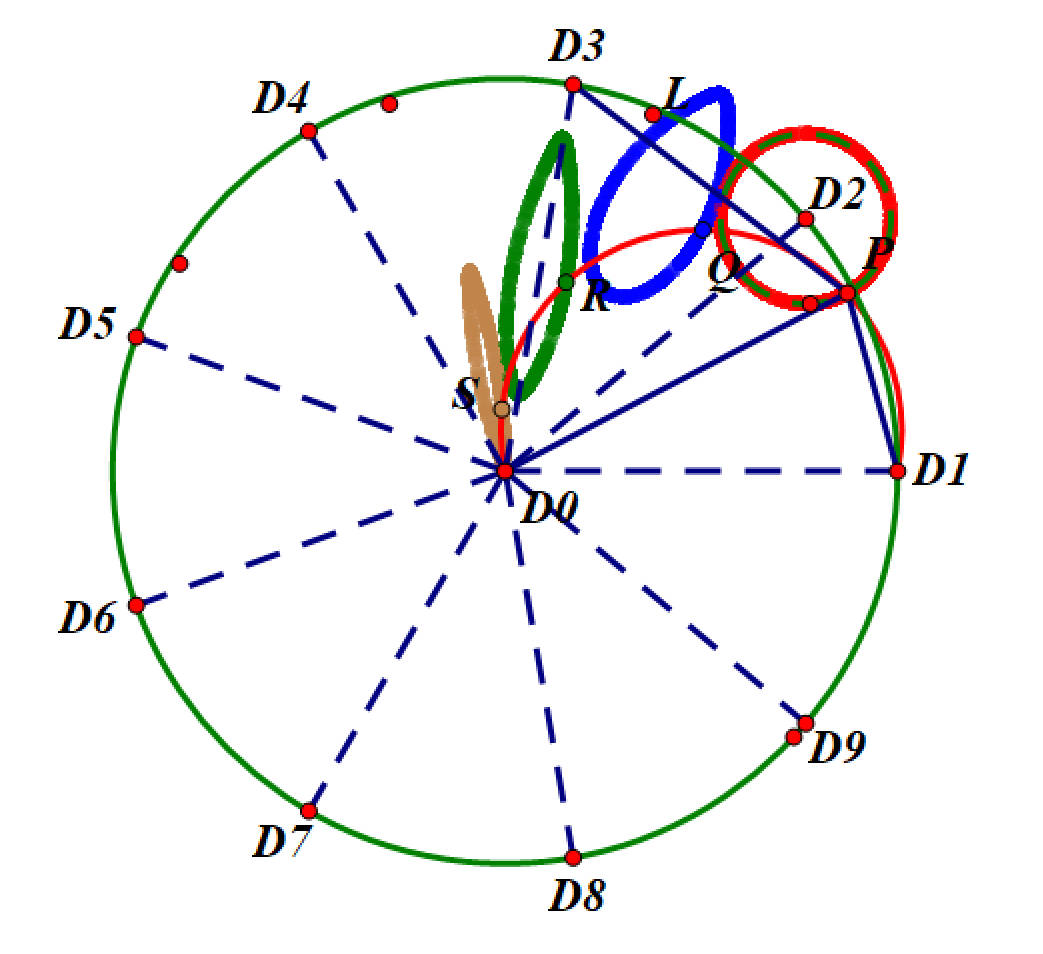
\includegraphics[width=0.2\linewidth]{../figures/8}}
				\\
				\subfloat[$r_0$很大时的运动轨迹情况]{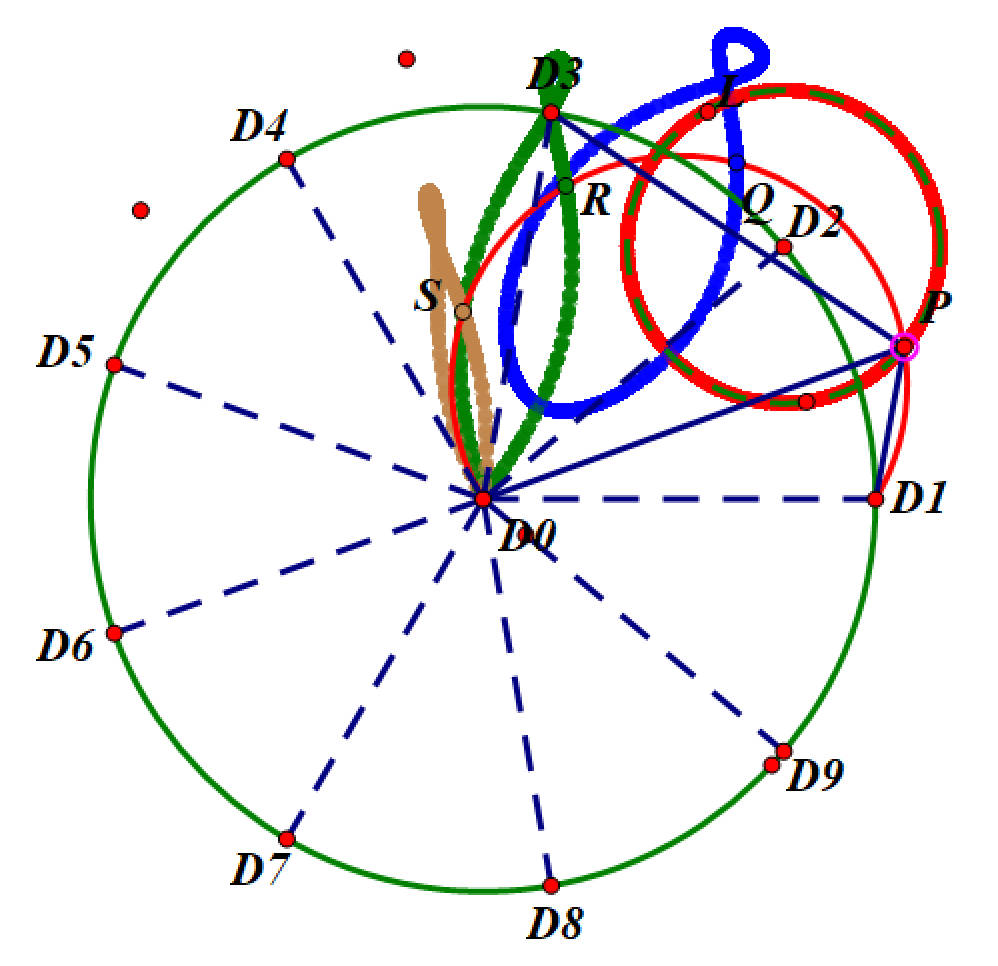
\includegraphics[width=0.2\linewidth]{../figures/9}}
				\caption{不同$r_0$的取值下$\mathcal{P}\text{(红)}\text{、}\mathcal{Q}\text{(蓝)}\text{、}\mathcal{R}\text{(绿)}\text{、}\mathcal{S}\text{(棕)}$的边界分布}
				\label{fig7}
			\end{figure}
			从图\ref{fig7}可以看出,$r_0$很大时,$\mathcal{P}\text{、}\mathcal{Q}$的边界有重叠,即$
			\exists p\in \mathcal{P},\ q\in \mathcal{Q}\ \ s.t.\ \left| \overrightarrow{pD_2} \right|\ >\left| \overrightarrow{qD_2} \right|$ 此时根据如果根据预测点到理想点最近的原则确定匿名无人机编号,将会误认为是$D_4$发射的信号,进而将自己的位置误认为$q$的位置。如图\ref{fig4}所示。
			
			我们希望存在一个最大的$r_2$,当$\lVert\omega_i\rVert \leqslant r_2$时,从正确的匿名无人机得到的解一定是所有可能解中距离理想位置最近的一个,从而使用最近点原则找到正确的发射源。
			
			使用动态几何求解器,我们求得在上述情形下$\mathcal{P}\text{、}\mathcal{Q}$边界相切时,$r_{2max}\approx 0.228\left| \overrightarrow{D_0D_1} \right|$。
			进一步,我们探索了匿名无人机变化与边界情况$r_i$的最大取值之间的关系。我们得出结论:$r_i$的最大取值与匿名无人机的的变化无关,只与待测无人机的编号i有关。
			\begin{figure}[H]
				\centering
				\subfloat[匿名无人机为$D_3$时的边界情况]{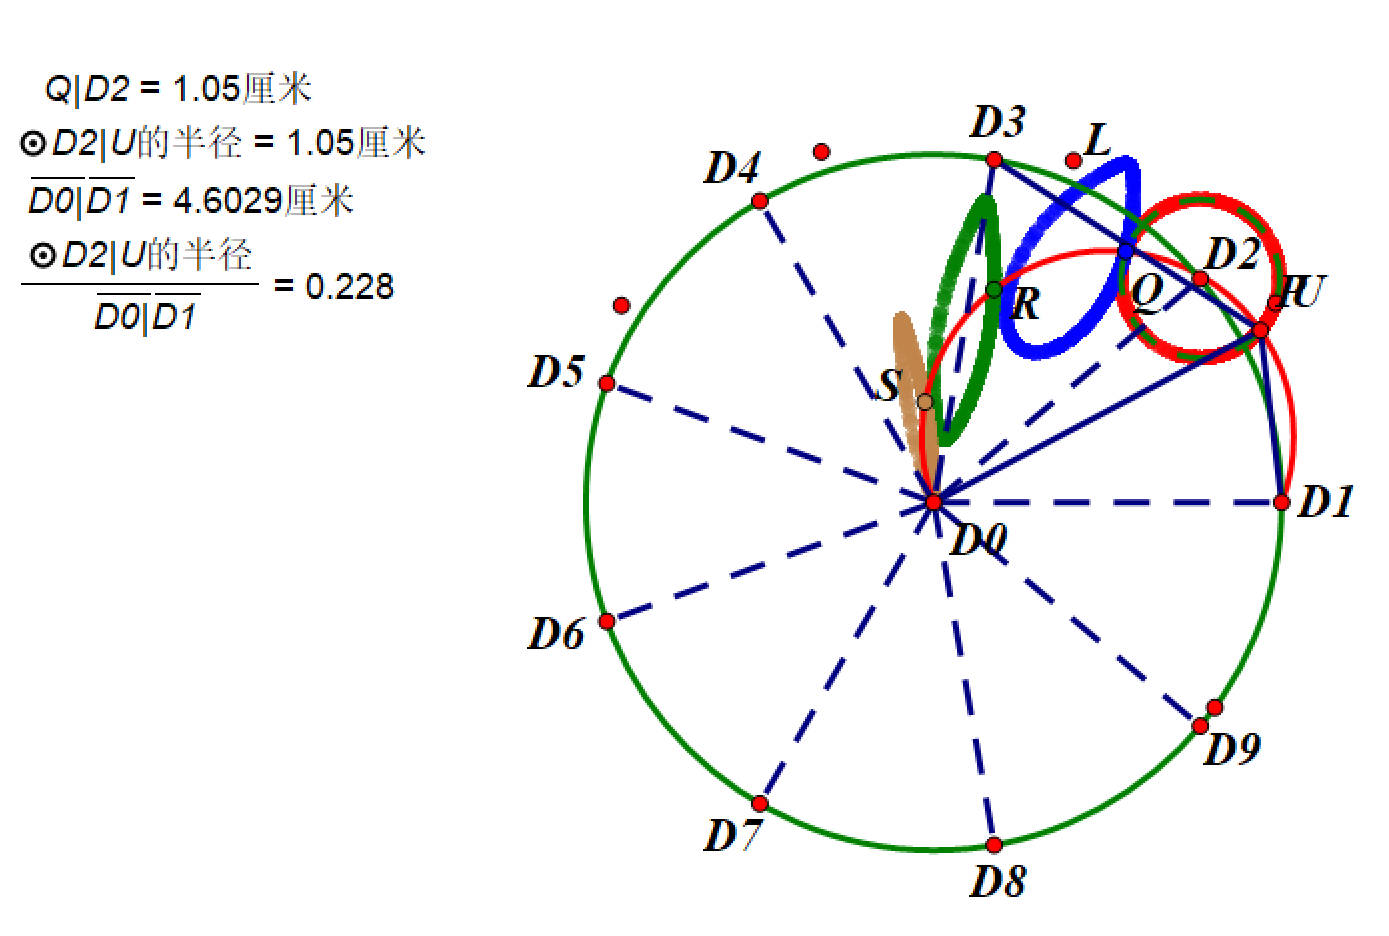
\includegraphics[width=0.45\linewidth]{../figures/10}}
				\subfloat[匿名无人机为$D_4$时的边界情况]{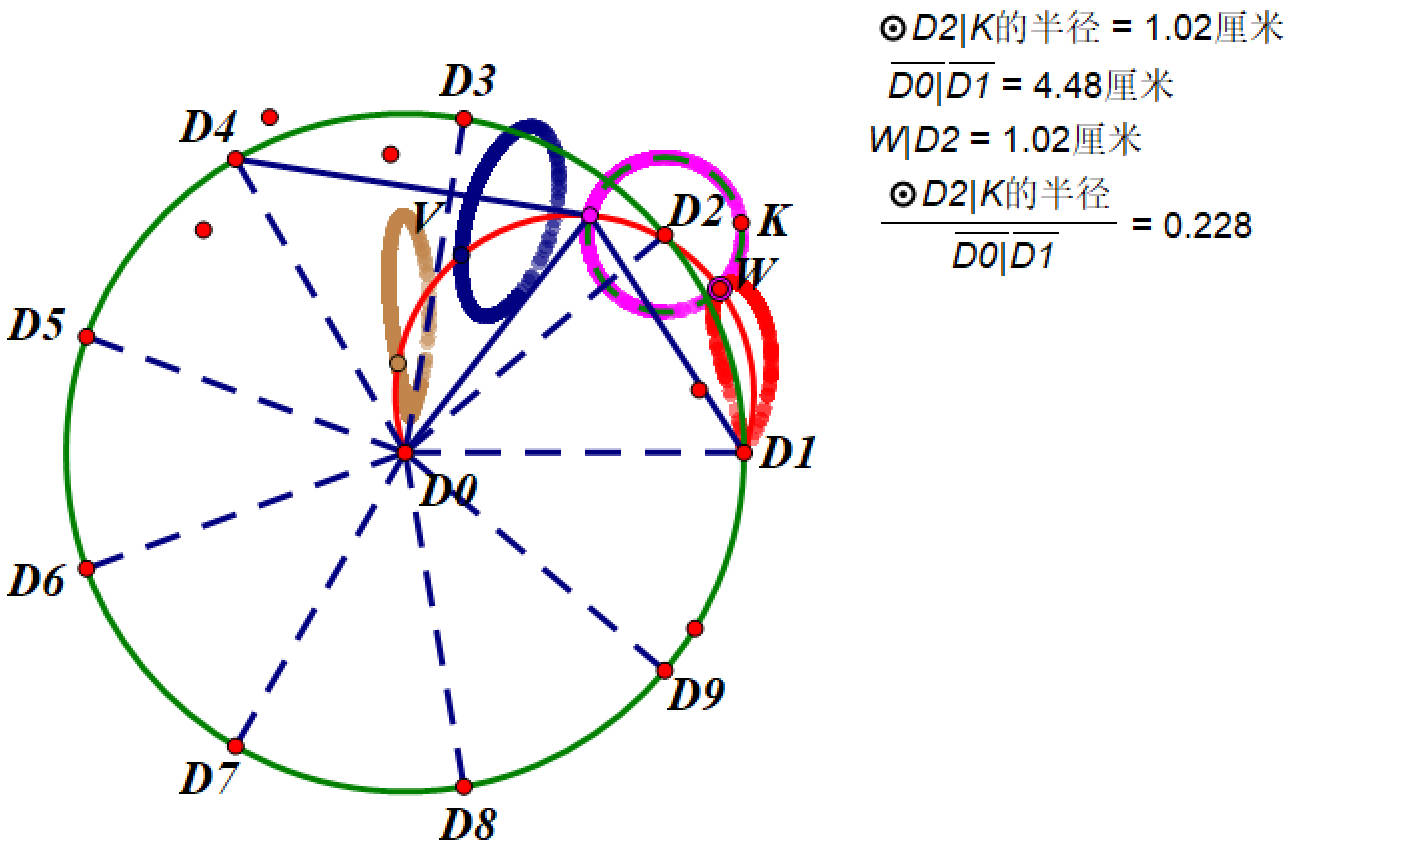
\includegraphics[width=0.45\linewidth]{../figures/11}}
				\caption{不同匿名无人机情况对于$D_2$唯一解边界情况的影响}
				\label{fig10}
			\end{figure}
		
			进一步,我们探索了不同待测无人机的最大误差范围。
			根据我们的模拟,我们有如下临界情况,见图\ref{fig12}.
			\begin{figure}[htb]
				\centering
				\subfloat[待测无人机为$D_3$时的边界情况]{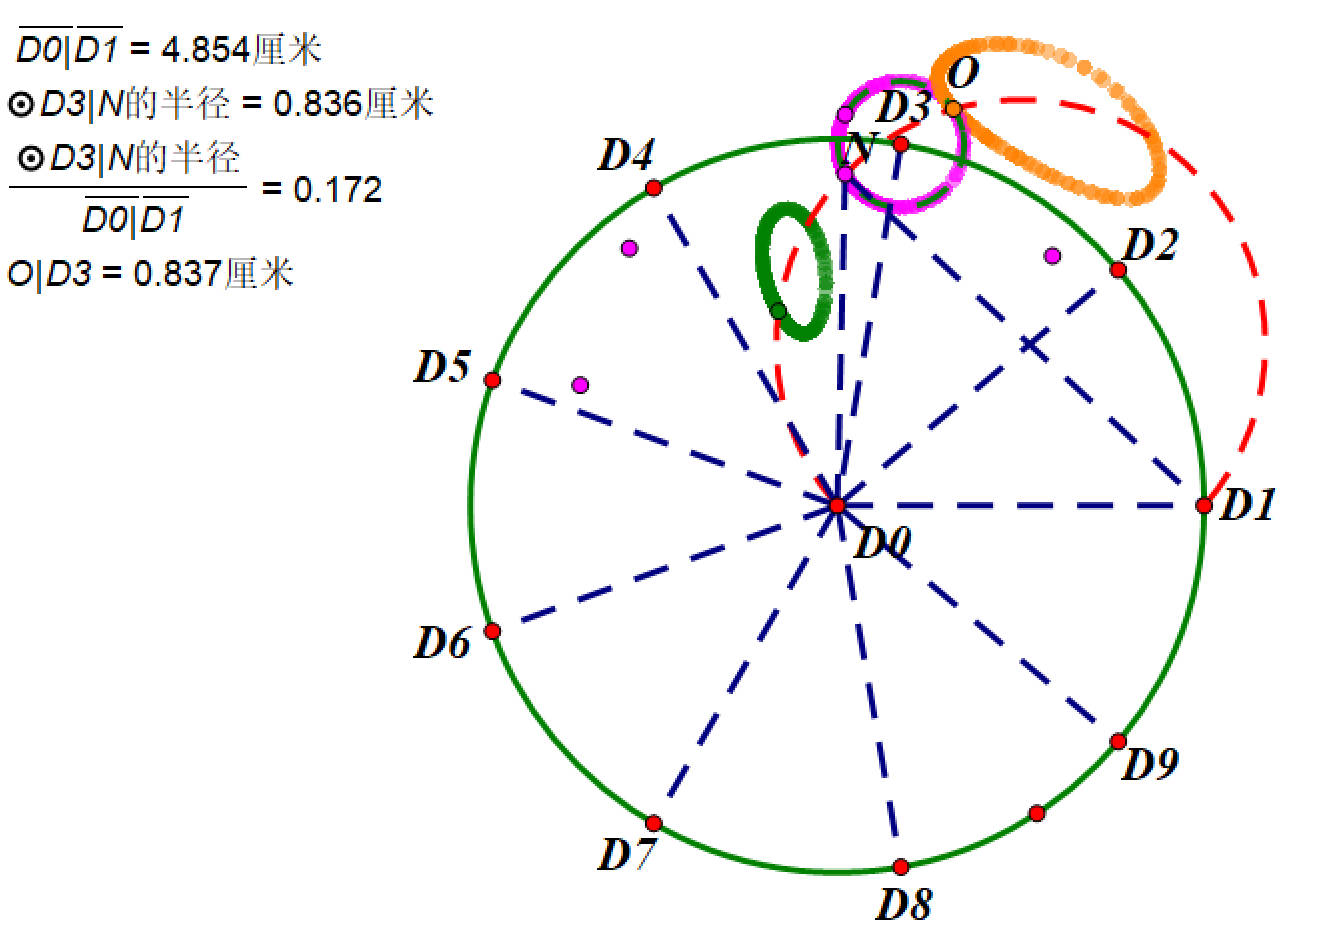
\includegraphics[width=0.45\linewidth]{../figures/12}}
				\subfloat[待测无人机为$D_4$时的边界情况]{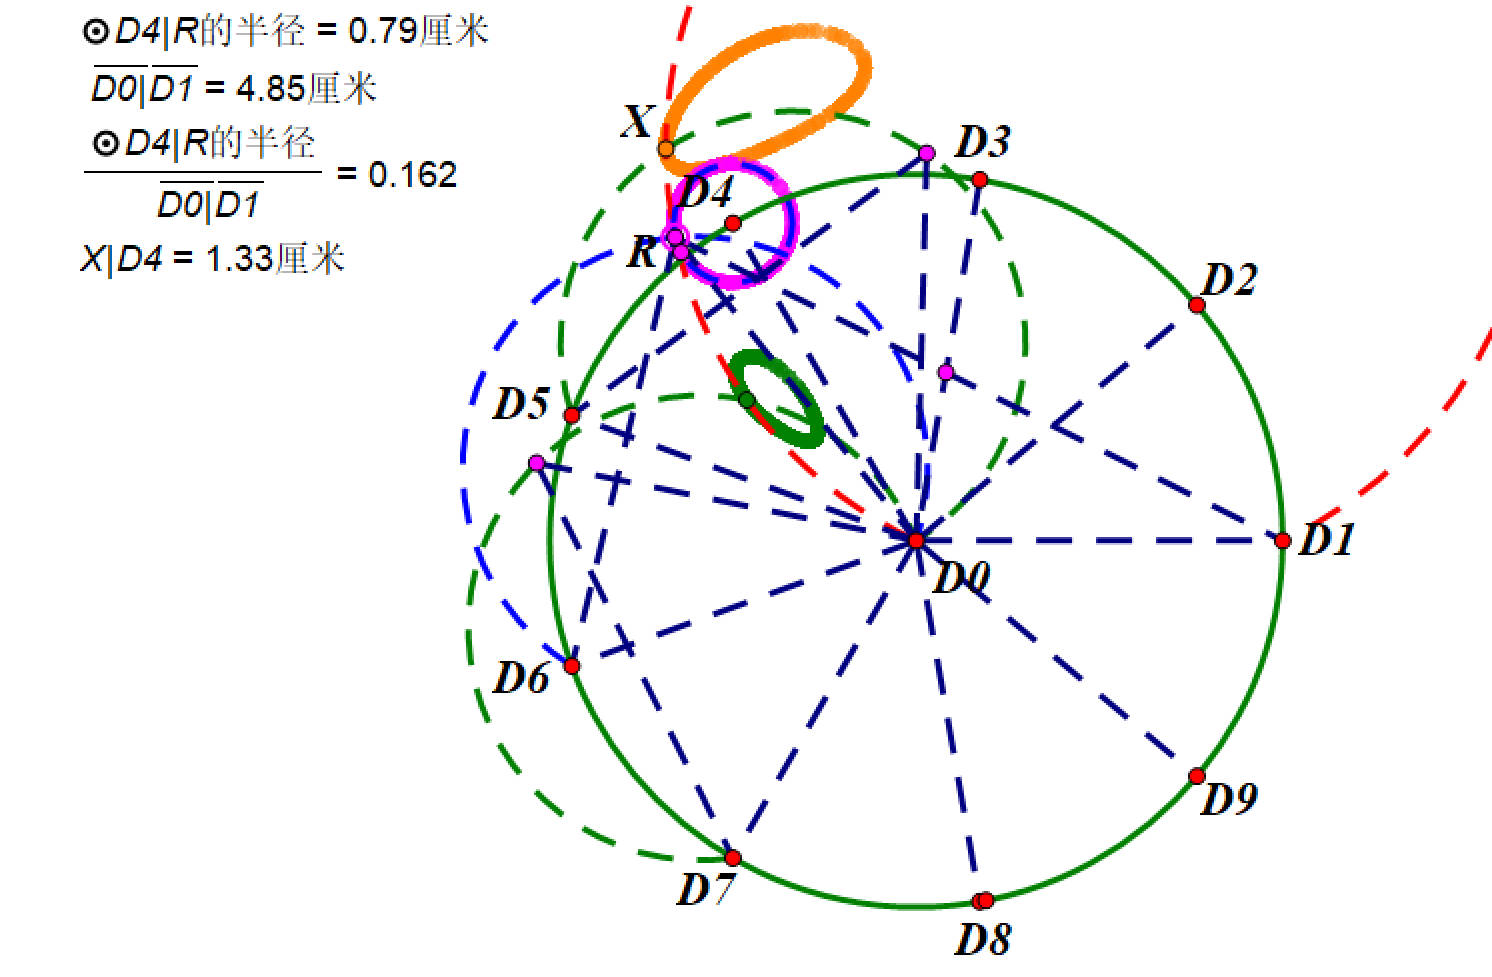
\includegraphics[width=0.5\linewidth]{../figures/13}}
				\\
				\subfloat[待测无人机为$D_5$时的边界情况]{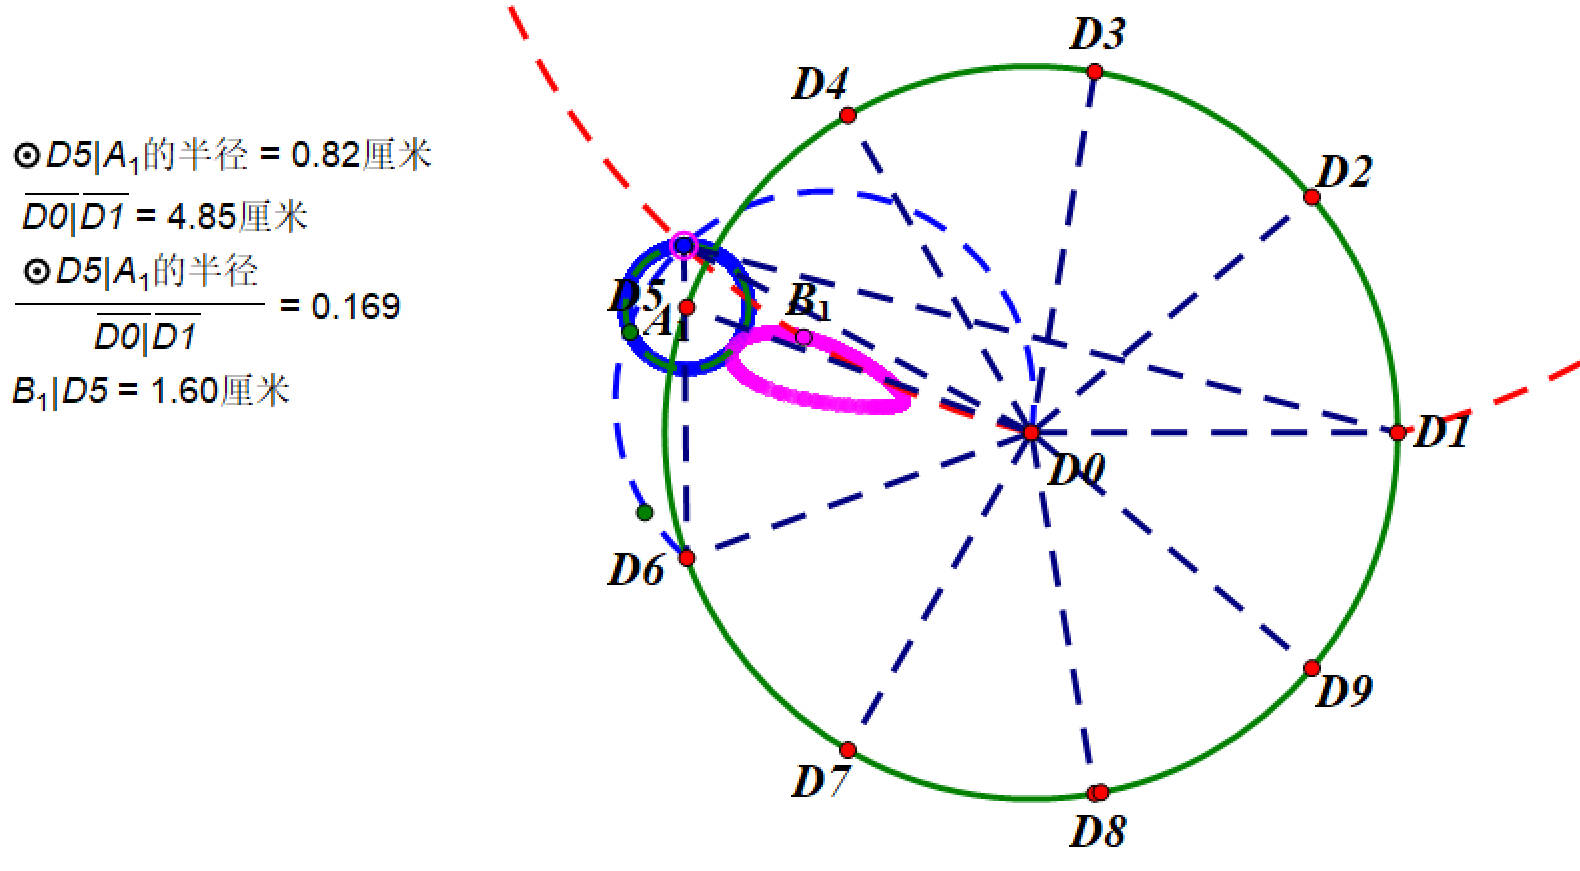
\includegraphics[width=0.55\linewidth]{../figures/14}}
				\caption{不同待测无人机唯一解边界情况}
				\label{fig12}
			\end{figure}
			\par
			令$r_i$为第i个无人机作为待测无人机时,有单一解时$\overrightarrow{\widehat{D_i}D_i}$的模长。
			我们分别得出,$r_{3max}\approx 0.172\left| \overrightarrow{D_0D_1} \right|,r_{4max}\approx 0.162\left| \overrightarrow{D_0D_1} \right|,r_{5max}\approx 0.169\left| \overrightarrow{D_0D_1} \right|$。
			根据对称性,我们同理可得$D_6,D_7,D_8,D_9$分别为待测无人机的情况。
			
			综上,我们进而给出对于任意的无人机,其“偏差较小”的数学定义为$|\overrightarrow{\widehat{D_i}D_i|}<0.162|\overrightarrow{\widehat{D_0}D_1}|$。若知道具体编号,则可以适用不同的边界情况数据。
			
			观察第三问中给出的数据,发现所有的无人机有偏位置坐标均符合我们对于“偏差较小”的定义,我们认为此定义适用于本题的所有情形。
			
			综上,在合理定义“较小偏差”后,当所有无人机的位置符合的情况下,我们即可利用上述原则确定匿名第三者,进而使用第一问中的结论就可求得待求无人机的位置。
			
			\paragraph{对于圆上两个无人机定位充要性的论证}
			本部分在开头即提出了我们的结论,即圆上两架无人机就可以确定任何一个无人机的位置。其证明将会从必要性和充分性两个方面进行说明。
			\begin{itemize}
				\item	首先在本题的题设中,圆上均匀分布着9个无人机,不存在任意两架无人机与圆心共线的问题。
				\item	必要性:从前面的论证易得,使用一架圆周上的无人机与圆心配合时,此时待测无人机只能测到一个角度,此时的解空间即为定弦与定角所确定的圆弧,不能确定无人机的位置。
				\item	充分性:在“较小偏差”的唯一解定义下,使用两架无人机进行测量,可以使用算法排除多解情况,此时位置被唯一确定,因此两架圆上无人机的定位是充分的。
			\end{itemize}
			
		\subsection{问题一(3)}
			\par 我们将问题一(3)分为两个子问题:
			\begin{itemize}
				\item 选择发射信号飞机数量
				\item 设计无人机编队位置调整方案
			\end{itemize}
			下面分别对两个问题进行解答。
			\subsubsection{选择发射信号飞机数量}
			基于问题一,除去圆心编号为FY00的无人机外,至少还需要2架圆上的飞机,才能实现其余飞机的有效定位。在题目限制的条件下,我们可以选择的2架飞机发射信号,或选择3架飞机发射信号。通过对以下因素的分析,我们可以发现,选择3架飞机发射信号明显优于选择2架飞机发射信号:
			\begin{itemize}
				\item 定位误差
				\item 迭代次数
				\item 总电磁信号发送次数:基于电磁静默原则,总电磁信号发送次数尽可能越小越好。其值为:发射信号无人机数量$\times$迭代调整次数
			\end{itemize}

			
				\paragraph{双机定位与三机定位的误差分析}
			如图\ref{fig16}所示,我们将定位每一轮次中的定位情形作此抽象。对于发射信号的三架无人机$D_2,D_5,D_8$,有其实际位置$\widehat{D_2}\in C_2,\widehat{D_5} \in C_1,\widehat{D_8}\in C_3$,$C_1,C_2,C_3$为对应无人机的“微小偏差”区域(比例有所夸张),同时有待定位的无人机$\widehat{D_3}$,此时待定位无人机共能测得三个夹角$\angle \widehat{D_5}\widehat{D_3}D_0$,$\angle D_0\widehat{D_3}\widehat{D_8}$,$\angle \widehat{D_8}\widehat{D_3}\widehat{D_2}$。此时选取其中两个无人机就可以使用上述方法确定D的坐标,此时的三个测量值记为$D_{30},D_{31},D_{32}$。在双机定位的情况下若测量结果为$D_{30}$,此时的误差就是$|\overrightarrow{\widehat{D_3}D_{30}}|$,而在三机定位的情况下,存在一定概率使$\overrightarrow{\widehat{D_3}D_{30}}+\overrightarrow{\widehat{D_3}D_{31}}+\overrightarrow{\widehat{D_3}D_{32}} < min\{\overrightarrow{\widehat{D_3}D_{30}},\overrightarrow{\widehat{D_3}D_{31}},\overrightarrow{\widehat{D_3}D_{33}}\}$从而降低误差。
			\begin{figure}[H]
				\centering
				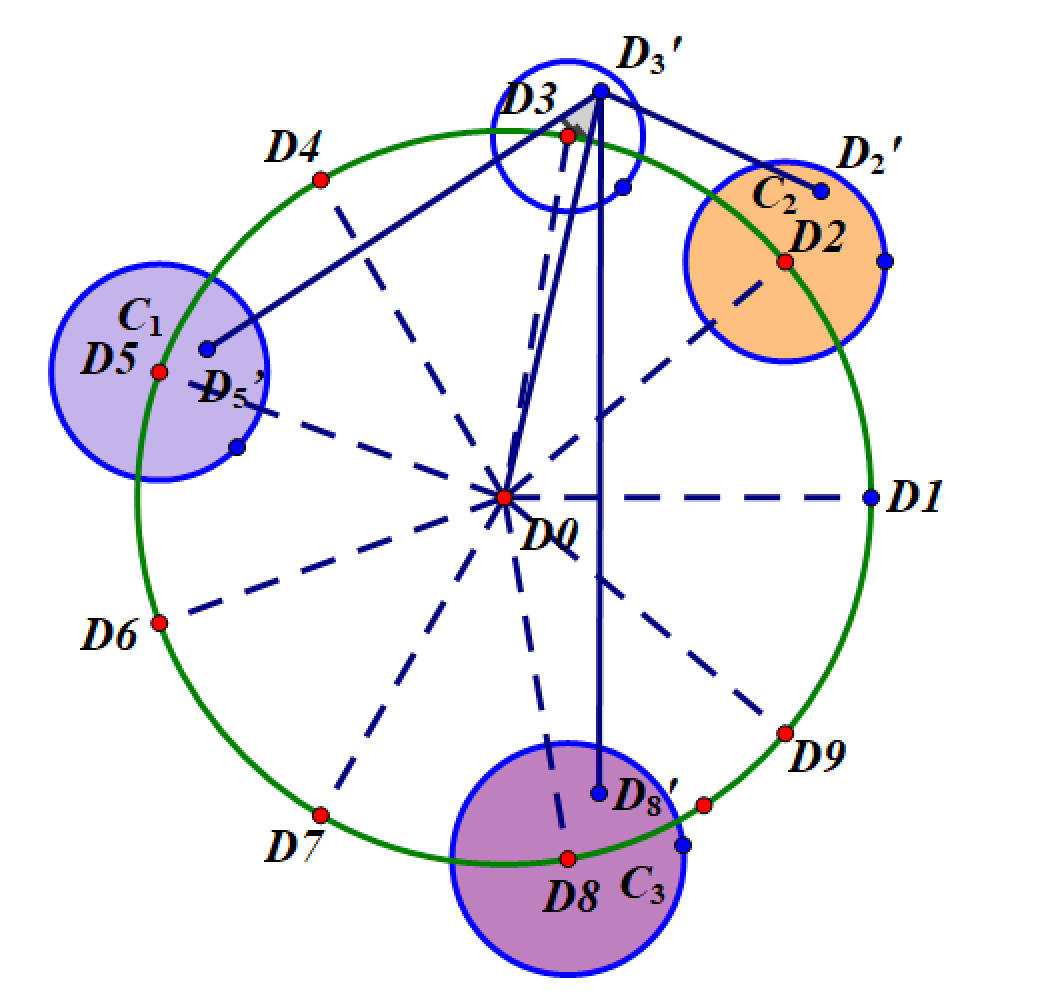
\includegraphics[width=0.3\linewidth]{./figures/16}
				\caption{定位问题的数学抽象}
				\label{fig16}
			\end{figure}
			不可否认的是,在此种情况下,亦存在$\overrightarrow{\widehat{D_3}D_{30}}+\overrightarrow{\widehat{D_3}D_{31}}+\overrightarrow{\widehat{D_3}D_{32}} > min\{\overrightarrow{\widehat{D_3}D_{30}},\overrightarrow{\widehat{D_3}D_{31}},\overrightarrow{\widehat{D_3}D_{33}}\}$的情况,为了验证本方法是否可行,对于使用计算机对于随机情况进行统计分析。
			\begin{figure}[H]
				\centering
				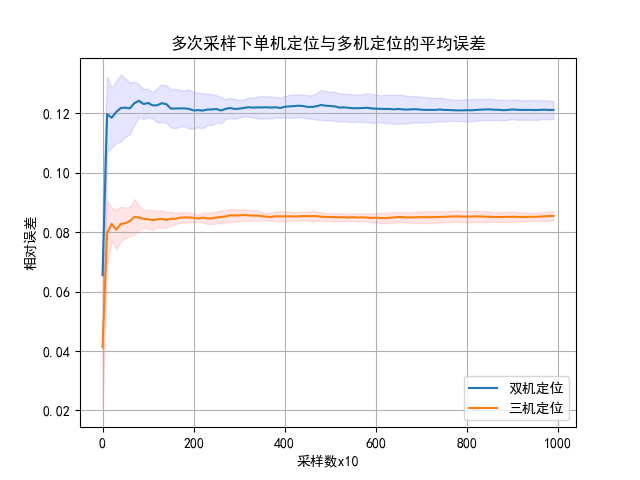
\includegraphics[width=0.45\linewidth]{./figures/15}
				\caption{多次采样下双机与三机系统的平均误差}
				\label{fig15}
			\end{figure}
			经过1000次随机采样,使用双机与三机系统对圆上每个点进行位置计算的平均误差如图\ref{fig15}所示。经统计分析,在双机系统进行位置计算时,平均误差约为$0.12R$,而使用多机系统时,平均误差降至$0.086R$,有$28.3\%$的性能提升。
		
			\subsubsection{无人机编队位置调整方案}
			我们定义一次迭代过程为:1.选择3架无人机与编号为FY00的无人机一起发射信号,2.其余无人机接收信号并定位位置,3.其余无人机进行位置调整。从初始情况开始,通过多次迭代,将机群调整为理想分布。
			\paragraph{选择发射信号无人机}
			根据5.3.1节的分析,我们每次选择理想位置将圆三等分的三架无人机发射信号,采用轮流的方式,第1次采用FY01、FY04、FY07,第2次采用FY02、FY05、FY08,第3次采用FY03、FY06、FY09...进行发射信号。
			\begin{figure}[htb]
				\centering
				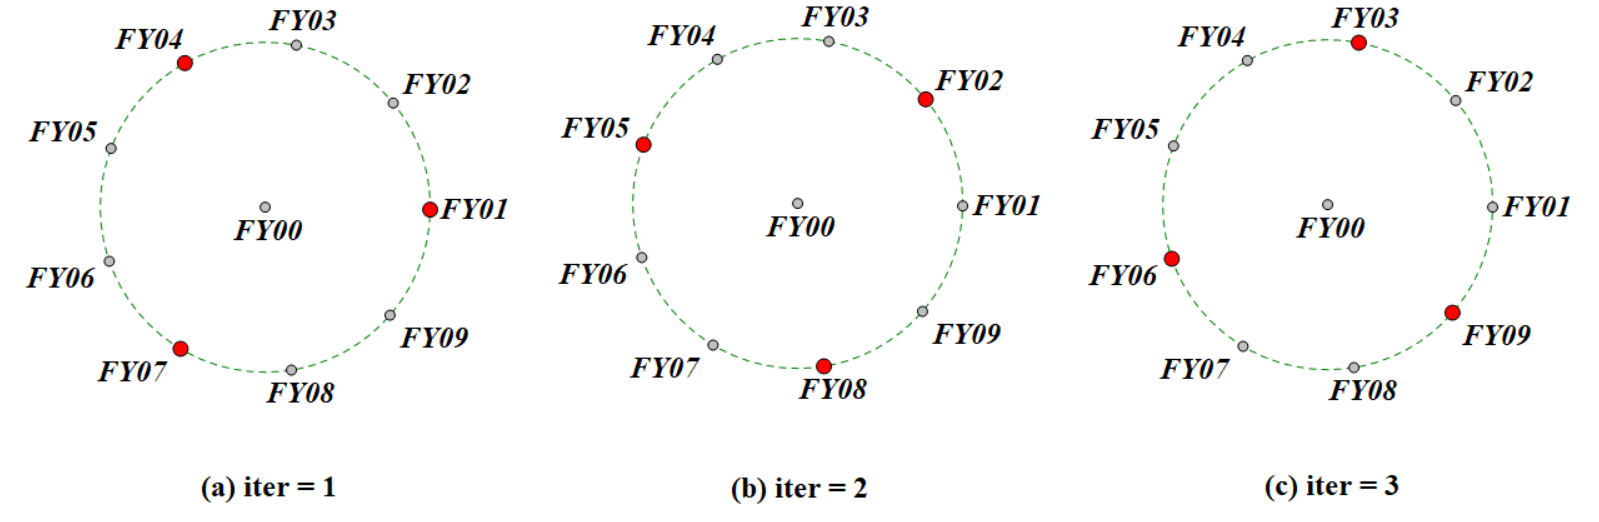
\includegraphics[width=1.0\linewidth]{./figures/发射信号无人机示意图}
				\caption{发射信号无人机选择示意图(图示位置为理想位置)}
				\label{发射信号飞机}
			\end{figure}
			\paragraph{无人机定位}
			对圆上无人机,出去发射信号的无人机,识别出接收信号的来源,该问题变成了利用编号FY00无人机与圆上3架确定编号的无人机进行定位的问题。记定位得到测量位置$(x_{measure},y_{measure})$,根据问题一,取其中2个发射信号可以得到定位,共有$C^2_3=3$种结果,如下所示:
			$$(x_{measure}^1,y_{measure}^1),(x_{measure}^2,y_{measure}^2),(x_{measure}^3,y_{measure}^3)$$
			对3个测量位置取平均,得到结果飞机的位置估计$(\hat{x},\hat{y})$:
			$$
			\left\{ \begin{array}{l}  \hat{x}=\sum_{i=1}^3{x_{measure}^{i}}\\  \hat{y}=\sum_{i=1}^3{y_{measure}^{i}}\\ \end{array} \right.  
			$$
			
			\paragraph{无人机位置调整}
			定义偏差$w$为无人机理想位置与估计位置的偏差:$\boldsymbol{w}=(x_{ideal},y_{ideal}) - (\hat{x},\hat{y})$,设置参数$\eta{}$,以$\boldsymbol{w}$作为位移调整位置,调整后的位置$(x_{new},y_{new})$为:$(x_{new},y_{new})= (x_{actual},y_{actual}) - \eta{} * \boldsymbol{w}$。
			\par 调整结果如下图\ref{Polar}所示,可以看到调整后的各个无人机较为均匀的分布在统一圆周上:
			\begin{figure}[H]
				\centering
				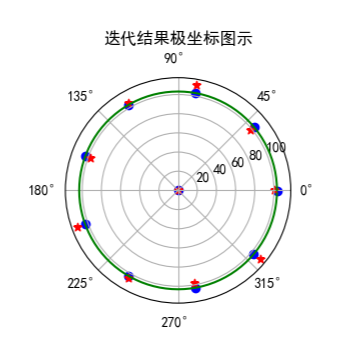
\includegraphics[width=0.35\linewidth]{./figures/Polar Axis}
				\caption{迭代调整后的结果对比图}
				\label{Polar}
			\end{figure}
	
		
			\paragraph{调整方案伪代码}
			调整方案的伪代码如下所示:
			\par
			\begin{algorithm}[H]
				\caption{无人机迭代调整算法}
				\KwIn{无人机的初始位置信息$UAV_{initial}$, 被动接受的方位信号$\alpha_1\text{与}\alpha_2$ }
				\KwOut{调整完成的最终位置信息$UAV_{hat}$}
				初始化算法的超参数:最大迭代次数$ maxIter $、学习率$ \eta $、迭代权重系数$ weight $;
				\par \For{$iter=start;iter \le maxIter;iter++$}
				{
					\#选择三架分布均匀的无人机作为一组承担发射信号的任务。
					\par  $ launch[i] =(launch[i-1] + 3) \% 9 $
					\par \For{$ i\ in range(1,10) \text{且} i ≠ launch[i] $ }
					{
						计算三架无人机中任意两架与待定位无人机的夹角 $\alpha[i],i=1,2,3 $ \;
						进而转化为第一问的情况可以计算三组测量坐标
						\par $ Compute\quad the\quad position\_measure\_list $
						\par \#将测量坐标求取均值以获得一组最终估计坐标
						\par  $ position\_estimate= Mean(position\_measure\_list) $
						\par \#计算估计坐标与理想坐标的误差
						\par$  error = ideal\_xy -position\_estimate $
						\par \#利用计算所得误差进行位置坐标的更新
						\par \If{$position\_estimate[i] < 0 or > 0 $}
						{
							\# 通过估计坐标的$ x,y $坐标的正负判断所在象限
							\par replace $position\_estimate$ with $ PolarAxisPosition $;
						}
					}
					\# 绘制初始极坐标和调整后极坐标示意图;		
				}
				\textbf{Return:}返回迭代后的无人机的 $postion$;
				\label{code1}
			\end{algorithm}
			\paragraph{对于一种特殊情况的讨论}
		在建模的过程中,我们意识到了一种特殊情况如图\ref{fig17},此时所有圆上的无人机都均匀分布或近似均匀分布在圆上,但圆心$D_0$偏移到了$\widehat{D_0}$的位置,此时也可以使用上述方法进行调整,使新圆的圆心为$\widehat{D_0}$。然而,此时最有的调整方案应该是移动圆心的位置使其回到$D_0$,但是考虑到本题需要在每次令中心无人机发射信号,\textbf{其余}无人机接收信号,中心无人机不能获取自身的位置信息,所以调整圆心的方案不可行。
		\begin{figure}[H]
			\centering
			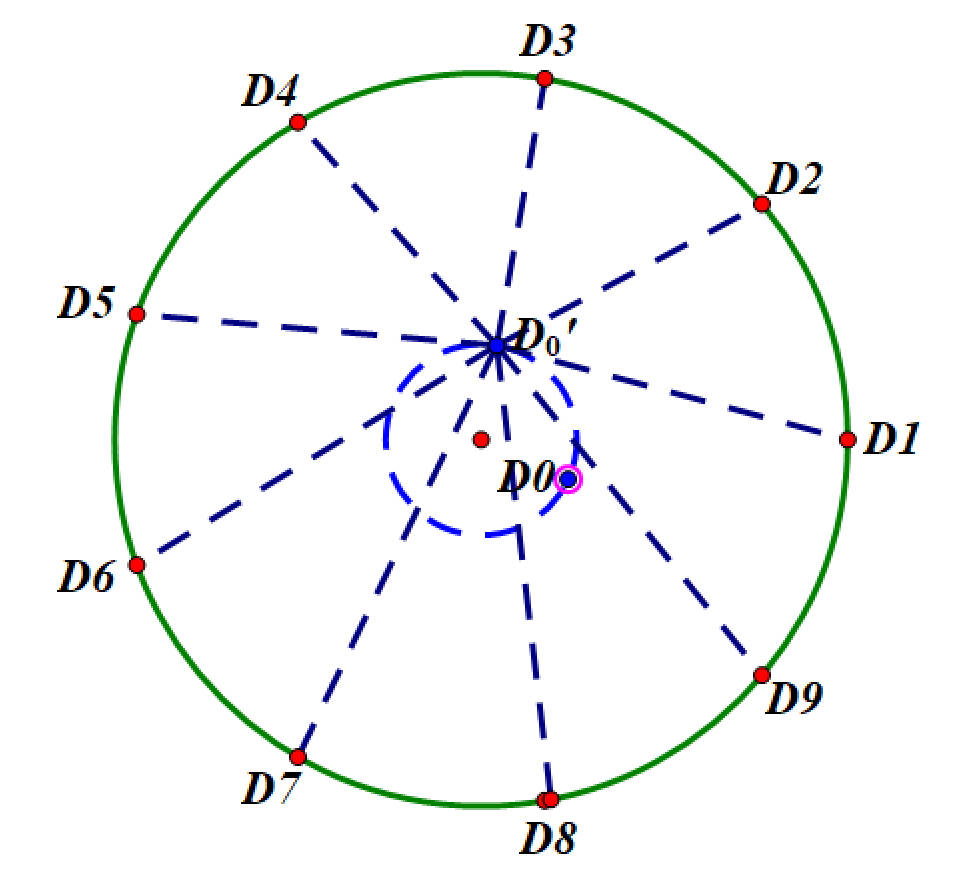
\includegraphics[width=0.35\linewidth]{./figures/17}
			\caption{圆心偏移的特殊情况}
			\label{fig17}
		\end{figure}
		\subsection{问题二}
		将问题二分解为2个子问题:
		\begin{itemize}
			\item 非顶点无人机调整策略;
			\item 顶点无人机调整策略。
		\end{itemize}
		前者包含3个阶段,后者包含1一个阶段,共有4个阶段。
		\subsubsection{非顶点无人机调整策略}    
		我们采用逐区域调整的方法,如图\ref{非顶点}所示,按照“灰色区域$\longrightarrow{}$橙色区域$\longrightarrow{}$紫色区域”的顺序进行调整。经过该策略,我们得到除去无人机{FY11,FY01,FY15}外所有无人机的位置,我们对三个区域采用不同的方法进行调整,注意三个区域在几何上是等价的,但由于调整顺序和策略的不同,在求解中的地位是不等价的:
		\begin{figure}[htb]
			\centering
			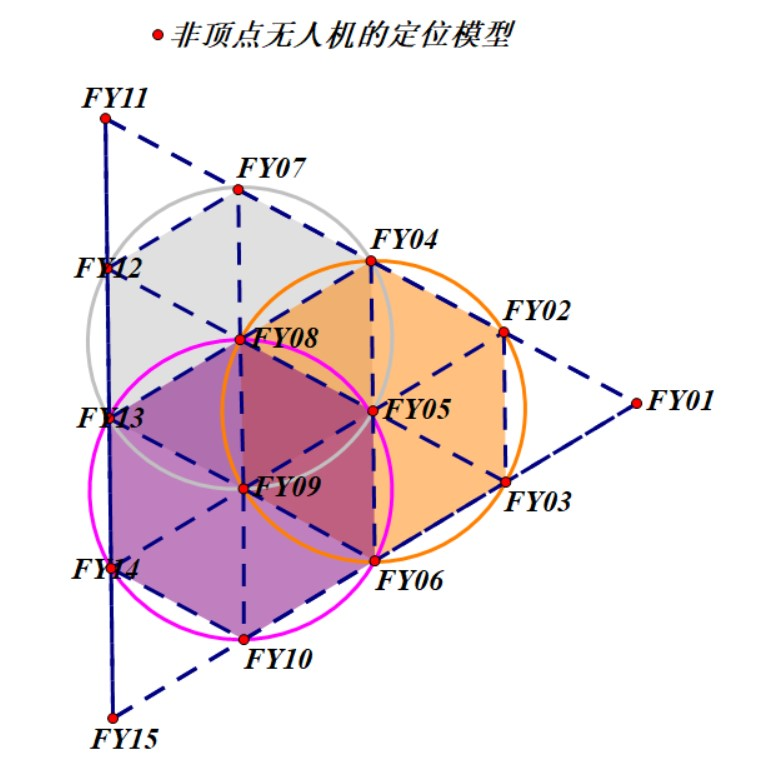
\includegraphics[width=0.55\linewidth]{../figures/非顶点定位}
			\caption{非顶点无人机定位模型}
			\label{非顶点}
		\end{figure}
		\paragraph{阶段一:灰色区域}作为第一个调整的区域,该圆上所有无人机、圆心处无人机的位置均与理想位置有所偏差,属于\textbf{发射信号无人机位置略有偏差的定位模型},与\textbf{问题一第(3)小问的情况相同},问题一第(3)小问的定位方法对灰色区域也同样适用,具体方法为:\\
		(1).按照发射信号飞机均匀分布原则,采用无人机FY07,FY13,FY05和圆心无人机FY08发射信号,对无人机FY04,FY12,FY09进行定位与位置调整;\\
		(2).按照轮流原则,采用第(1)步的被测无人机,即FY04,FY12,FY09与圆心无人机FY08一同作为发射信号的无人机,对无人机FY07,FY13,FY05进行定位与位置调整;\\
		(3).重复步骤(1)、(2),直到圆上无人机均匀分布,且与圆心无人机距离小于某一阈值,或达到最大迭代次数时停止迭代;\\
		(4).得到编号为{FY08,FY04,FY07,FY12,FY13,FY09,FY05}的位置调整结果。
		\paragraph{阶段二:橙色区域}:
		当阶段一结束后,橙色区域中无人机{FY08,FY04,FY05,FY09}的位置确定,且构成两个等边三角使得:$$|D_4D_5|=|D_8D_5|=|D_9D_5|,$$其中$D_i$表示编号为$i$的无人机位置。无人机{FY08,FY04,FY05,FY09}不再次进行调整,并发射信号供无人机{FY02,FY03,FY06}定位调整。此时,模型转化\textbf{ 圆上三架无人机与圆心无人机发射信号,发射信号飞机编号已知且位置基本无偏差定位模型},可以采用\textbf{问题一第(1)、(3)小问}的方法求解。
		
		\paragraph{阶段三:紫色区域}:
		当阶段二结束后,紫色区域内编号为{FY13,FY08,FY09,FY05,FY06}的无人机位置确定,作为发射信号无人机,编号已知且位置基本无偏差,无人机{FY14,FY10}进行定位并调整。具体方法为:\\
		(1).采用无人机FY13,FY08,FY09,FY05发射信号,对无人机FY14,FY10进行定位与位置调整;\\
		(2).为消除可能误差,再采用无人机FY06,FY08,FY09,FY05发射信号,对无人机FY14,FY10进行定位与位置调整;\\
		(3).重复步骤(1)、(2),直到圆上无人机均匀分布,且与圆心无人机距离小于某一阈值,或达到最大迭代次数时停止迭代;\\
		
		\subsubsection{顶点无人机调整策略}
		
		经过非顶点无人机调整策略,编队中仅有顶点无人机{FY11,FY01,FY15}的位置未确定,每架无人机都在两个以相邻无人机间隔为半径的圆上,如图\ref{顶点}。以无人机FY11为例,采用以下方法进行调整:\\
		\begin{figure}[htb]
			\centering
			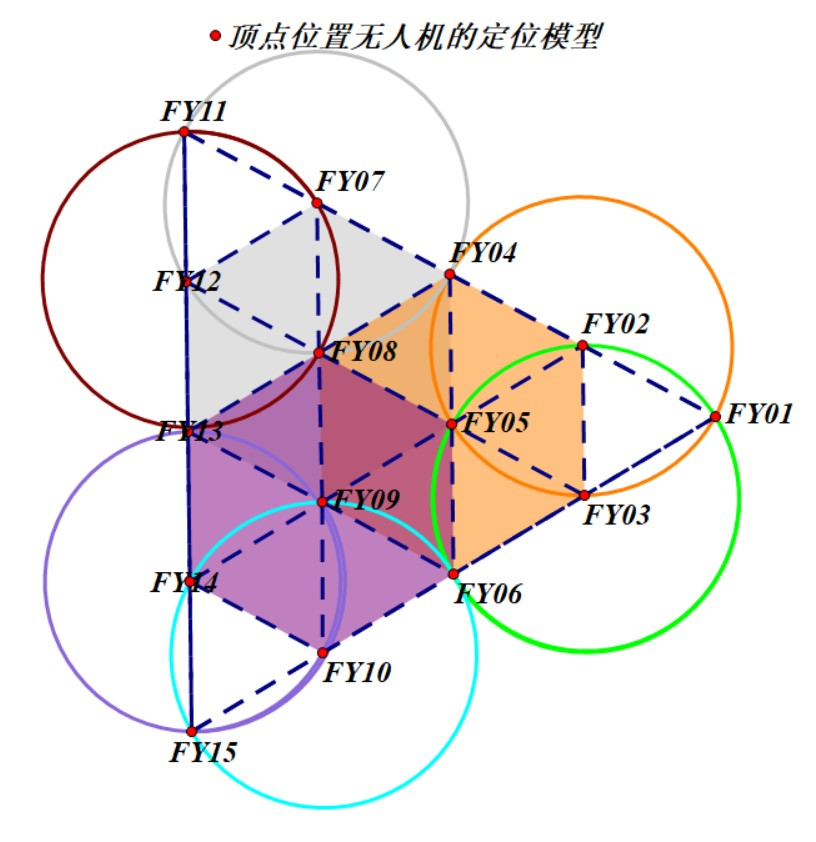
\includegraphics[width=0.55\linewidth]{../figures/顶点定位}
			\caption{顶点无人机定位模型}
			\label{顶点}
		\end{figure}
		(1).基于以无人机FY07为圆心的圆,采用无人机FY07,FY12,FY08,FY04发射信号,让无人机FY11进行定位与调整;\\
		(2).为减小误差,再基于以无人机FY12为圆心的圆,采用无人机FY07,FY12,FY08,FY13发射信号,让无人机FY11进行定位与调整;\\
		(3).重复步骤(1)、(2),直到圆上无人机均匀分布,且与圆心无人机距离小于某一阈值,或达到最大迭代次数时停止迭代;\\
		\subsubsection{调整方案伪代码}
		\begin{algorithm}[H]
			\caption{锥形编队式十六架无人机迭代调整算法}
			\KwIn{无人机的理想位置信息$UAV_{ideal}$,无人机阵列的邻接矩阵信息, 被动接受的方位信号$\alpha_1\text{与}\alpha_2$ }
			\KwOut{调整完成的最终位置信息$UAV_{hat}$,以及偏差评估值}
			\par 初始化算法的超参数:最大迭代次数$ maxIter $、学习率$ \eta $、迭代权重系数$ weight $;
			\par 通过添加随机高斯噪声生成实际位置和初始随机预估位置。
			\par 选定非顶点无人机作为初始圆心$ D_0 $(例如编号FY$ 08 $)
			\par \# 进而将问题转化为第一题第二问的定位模型\ref{code1}
			\par 基于第一次求解得到的无人机的位置的信息,我们便可以将其余非顶点无人机(如编号为FY$ 05$或FY$ 09 $)的无人机定位模型转化为第一题第一问的数学模型
			\par 最后仍选取非顶点无人机(如编号为FY$09$)作为圆心,利用第一问的数学模型求解
			\par \# 非顶点的无人机定位完成后,剩余三个顶点无人机
			\par 可利用已知信息选取两组$ position_{estimate} $,两次分别对其位置调整。
			\par \# 绘制初始极坐标和调整后极坐标示意图;		
			
			\textbf{Return:}返回迭代后的无人机的 $position$;
			\label{code4}
		\end{algorithm}
		\subsubsection{结果分析与展示}
		\paragraph{结果展示}
		对每架无人机,我们在其理想位置的上加上随机噪声,使其与理想位置略有偏差但偏离在最小误差半径范围内,作为问题的初始情景。采用调整算法,对问题加以仿真,调整结果如图\ref{锥形调整结果}所示:
		\begin{figure}[htb]
			\centering
			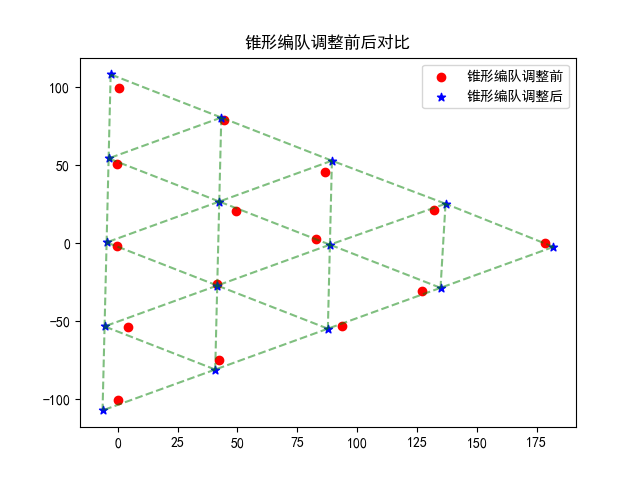
\includegraphics[width=1.0\linewidth]{../figures/Problem4}
			\caption{锥形无人机编队调整结果}
			\label{锥形调整结果}
		\end{figure}
		可以看到,调整后编队呈现正三角形,各无人机结点分布均匀,调整效果良好。
		\paragraph{结果分析}
		统计调整前、后编队相邻无人机间距(共30条边),计算方差、极差、均值等数据,结果如表\ref{调整效果}所示:
		\begin{table}[htb]
			\centering
			\begin{tabular}{|c|c|c|c|c|c|}
				\hline
				&标准差差&最大值&最小值&极差&均值\\
				\hline
				调整前&4.8848&62.7870&38.4652&24.3218&50.4069\\
				调整后&0.0018&50.7817&50.7910&0.0092&50.7856\\
				\hline
			\end{tabular}
			\caption{锥形编队调整前后指标}
			\label{调整效果}
		\end{table}
		可见通过调整,编队相邻无人机间距方差、极差大大减小,即编队拟合理想锥形分布的程度明显增加。另外,结合表\ref{调整效果}和图\ref{锥形调整结果}可知,调整相邻无人机间距的均值可能发生变化,且整体队形可能在原始对象上略有旋转,但编队拟合理想的锥形分布不构成影响,仍可以有很好的拟合效果
			
	\section{总结}
	\subsection{模型优点}
	\paragraph{(1).对于问题一第1小问}
	\par 
	采用极坐标表示方程,使方程形式简洁,同时容易设置合适初始值带入求解器求得数值解;\\
	\paragraph{(2).对于问题一第2小问}
	\begin{itemize}
		\item 模型直观,且能够运用计算机软件进行模拟;
		\item 能够在构建模型的过程中完成对两架飞机的充分性和必要性进行证明,科学严谨。
	\end{itemize}
	\paragraph{(3).对于问题一第3小问}
	\begin{itemize}
		\item 采用大量随机数据进行蒙特卡洛分析,保证了方法的理论可靠性;
		\item 通过选择圆心无人机和圆上另外3最大间隔无人机发射信号,很大程度上降低了被测无人机的定位误差,使得在很小的迭代次数下得到很好的理想编队拟合情况;
		\item 很小的迭代次数使得无人机群总发射电磁信号很小,提高无人机群隐蔽性,满足电磁静默原则;
	\end{itemize}
	\paragraph{(4).对于问题二}
	\begin{itemize}
		\item 将复杂问题进行分治,将复杂编队模型分块转化为前述问题中解决的圆形编队问题,降低了问题复杂性;
		\item 仅有非顶点无人机调整第一个阶段是发射信号无人机位置可能有偏差的,其余阶段发射信号无人机位置无偏差,结合问题一(1)结论,从理论上保证结果的可靠性。
	\end{itemize}
	\subsection{模型缺点}
	(1).限制了无人机与理想位置之间的偏差不会超过一定阈值,超过阈值后会出现多解甚至无解的情况,调度算法对部分偏差过大的极端情况还考虑较少;\\
	(2).问题二求解迭代次数较多,发射电磁信号较多,不利于保持电磁沉默。
	
	\subsection{讨论}
	在使用蒙特卡洛方法中,需要使无人机坐标均匀分布在误差圆内。若直接对坐标$(\rho,\theta)$进行均匀分布随机处理,得到的点落在中心的概率大于落在边缘的概率,如图\ref{m}所示。若对均匀分布函数开根号,得到的结果基本为误差圆内的均匀分布。
	\begin{figure}[H]
		\centering
		\subfloat[数据耦合]{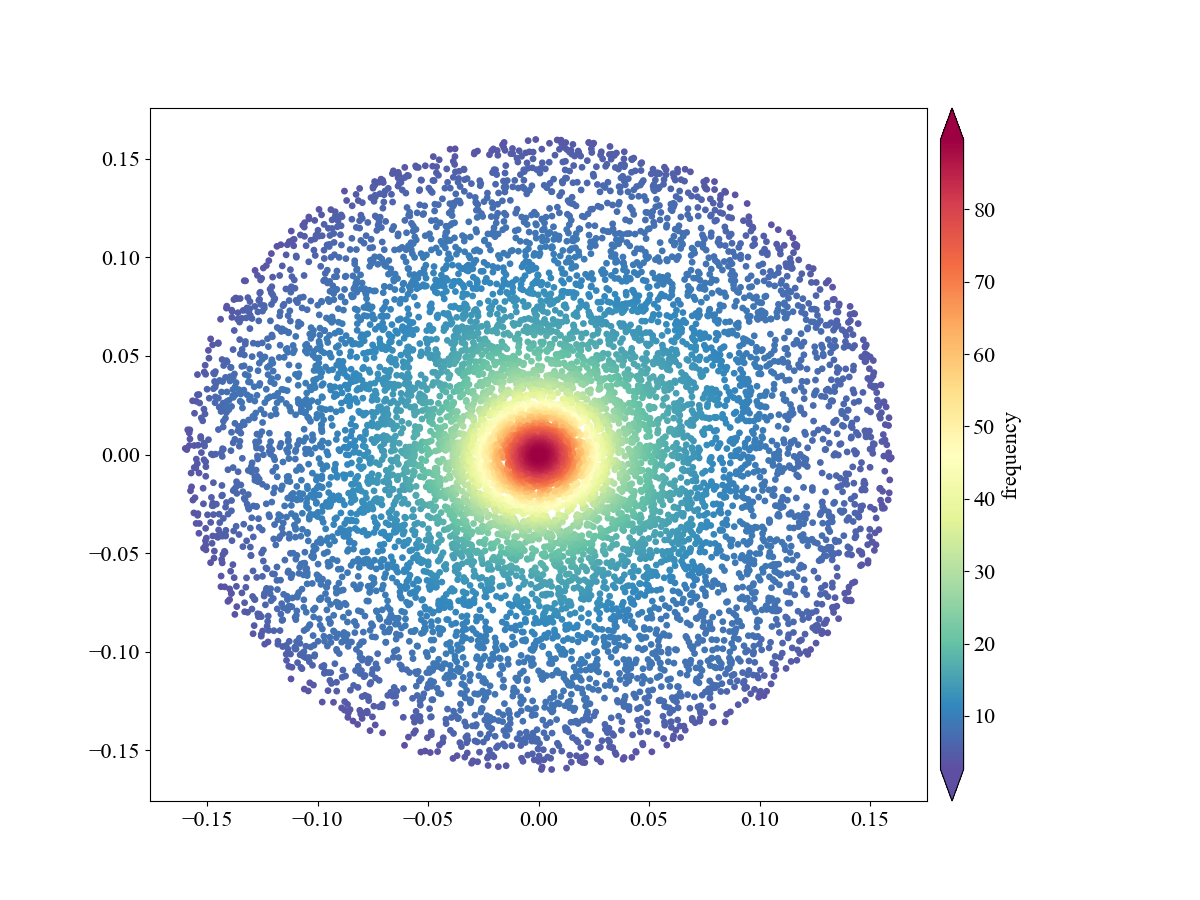
\includegraphics[width=0.45\linewidth]{./figures/m1}}
		\subfloat[数据去耦]{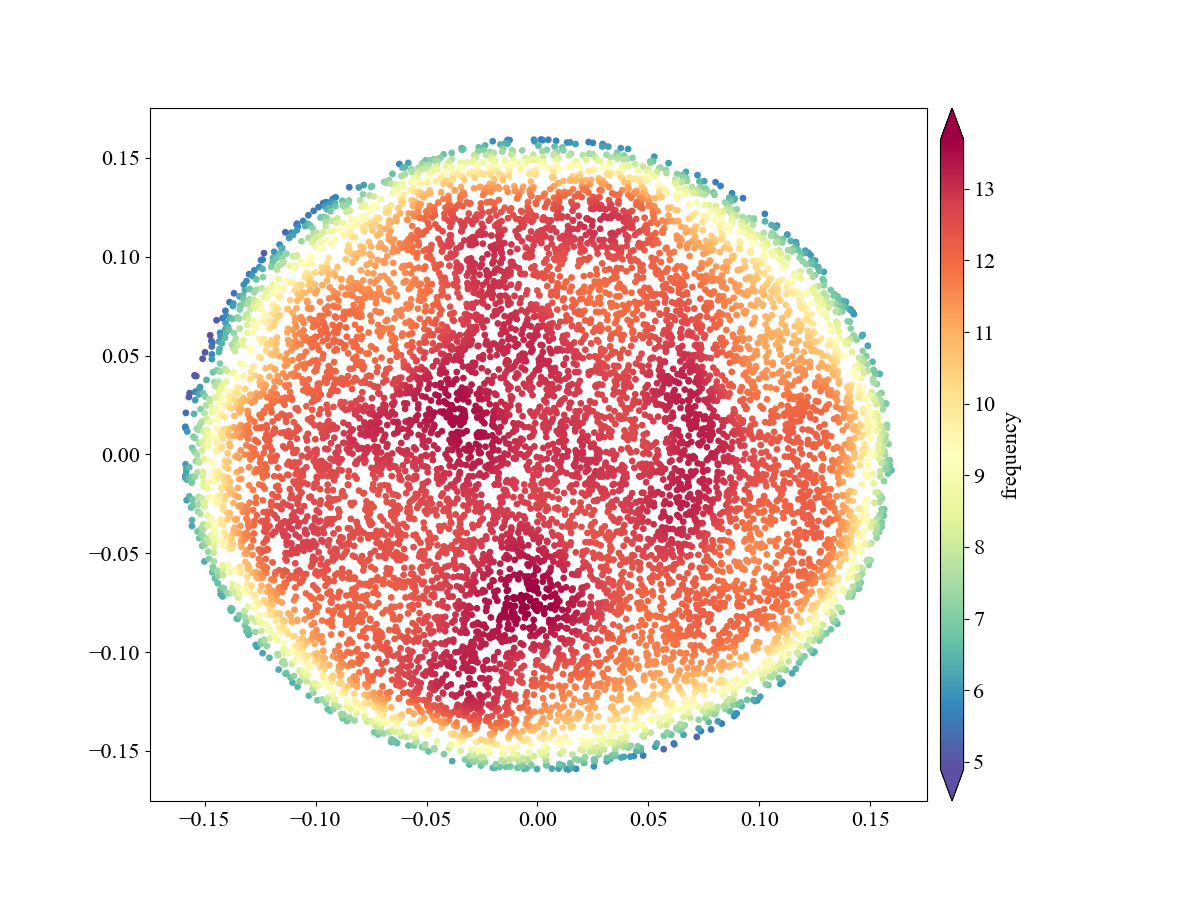
\includegraphics[width=0.45\linewidth]{./figures/m2}}
		\caption{不同随机生成方式对比}
		\label{fig meta}
	\end{figure}
	\bibliographystyle{unsrt}
	\bibliography{ref.bib}
	\section*{附录}
	\appendix
	\section{附录清单}
	\begin{itemize}
		\item 问题一主代码:平均圆规划与调整算法
		\item 问题二主代码:“定位-位移”迭代调整算法
		\item 问题二主代码:蒙塔卡洛法
	\end{itemize}
	\section{无源定位系统主算法代码}
	\subsection{问题一主代码:平均圆规划与调整算法}
	\begin{lstlisting}[language=python]
import numpy as np
import random
from scipy.optimize import root
from problem1 import get_angle,f_p2
from matplotlib import pyplot as plt

# 载入数据
plane = np.array([[0, np.deg2rad(0)], [100, np.deg2rad(0)], [98, np.deg2rad(40.10)],
[112, np.deg2rad(80.21)], [105, np.deg2rad(119.75)], [98, np.deg2rad(159.86)],
[112, np.deg2rad(199.96)], [105, np.deg2rad(240.07)], [98, np.deg2rad(280.17)],
[112, np.deg2rad(320.28)]])

plane_hat = plane
iter_max = 44
lr = 0.8
d = 100
fixed = 6
t = 0.5

position_remember_xy = np.zeros((10,2))

for iter in range(iter_max):
# 在1-9中随机选择一个无人机(不能是fixed),参与发射信号
while 1:
x = random.randint(1, 9)
if x != fixed:
break
# 发射信号,其余无人机得到角度
for i in range(1,10):
if (i == x) or (i == fixed):
continue

# 角度0-i-d=fixed
alpha_1 = get_angle(np.array([plane[0,:],plane[i,:],plane[fixed,:]]))
# 角度0ix
alpha_2 = get_angle(np.array([plane[0, :], plane[i, :], plane[x, :]]))

# 估算i的位置
angle = np.zeros(4)  # angle1,angle2,beta1,beta2
# alpha
angle[0] = alpha_1
angle[1] = alpha_2
# beta
angle[2] = (fixed - 1) * 2 / 9 * np.pi
angle[3] = (x - 1) * 2 / 9 * np.pi# 注意这个角是不知道的!!!!!!!!想办法改
ideal_angle = (i - 1) * 2 / 9 * np.pi
# 求相对坐标
# 注意相对坐标是指极径用相对值表示!!!!!!!!!!!!!!!!!!!!!!!!!!!!!!!!!!!!!!!!!!!!!!!
position = root(f_p2, [1, ideal_angle], args=(angle)).x
# 近似转化成绝对坐标
position[0] = position[0] * d
position_measure_xy = np.array([position[0] * np.cos(position[1]),position[0] * np.sin(position[1])])

# 首次更新记忆坐标
if not np.any(position_remember_xy[i,:]):
position_remember_xy[i, :] = position_measure_xy

position_esimate_xy = t * position_measure_xy + (1 - t) * position_remember_xy[i, :]

position_now_xy = np.array([plane[i,0] * np.cos(plane[i,1]),plane[i,0] * np.sin(plane[i,1])])
ideal_xy = np.array([d * np.cos(ideal_angle),d * np.sin(ideal_angle)])
w = ideal_xy - position_esimate_xy
# 位置调整
position_new_xy = position_now_xy + lr * w

# 更新记忆位置
position_remember_xy[i, :] = position_measure_xy + lr * w

# 得到角度
if (position_new_xy[0] >= 0) and (position_new_xy[1] >= 0): # 第一象限
a = np.arctan(position_new_xy[1]/position_new_xy[0])
elif (position_new_xy[0] < 0) and (position_new_xy[1] >= 0): # 第二象限
a = np.arctan(position_new_xy[1]/position_new_xy[0]) + np.pi
elif (position_new_xy[0] < 0) and (position_new_xy[1] < 0): # 第三象限
a = np.arctan(position_new_xy[1]/position_new_xy[0]) + np.pi
else: # 第四象限
a = np.arctan(position_new_xy[1]/position_new_xy[0]) + 2 * np.pi
plane_hat[i,:] = np.array([np.sqrt(position_new_xy[0]**2 + position_new_xy[1]**2),a])

print('/******************************************************/')
print('plane_hat')
print(plane_hat)


ax1 = plt.subplot(121, projection='polar')  #极坐标轴
# ax1.scatter(plane[:,1],plane[:,0],color='r')
ax1.scatter(plane_hat[:,1],plane_hat[:,0],color='b')
plt.show()


	\end{lstlisting}
	\subsection{问题二主代码:“定位-位移”迭代调整算法}
	\begin{lstlisting}[language=python]
		
		import random
		
		import numpy as np
		from matplotlib import pyplot as plt
		from scipy.optimize import root
		
		from problem1 import f_p2, get_angle
		
		plt.rcParams['font.sans-serif'] = ['SimHei']
		plt.rcParams['axes.unicode_minus'] = False
		
		
		def xy2polar(relative_xy):
		r=np.sqrt(np.dot(relative_xy,relative_xy))
		if (relative_xy[1] >= 0) and (relative_xy[0] == 0):
		theta = np.pi / 2
		elif (relative_xy[1] < 0) and (relative_xy[0] == 0):
		theta = np.pi / 2 * 3
		elif (relative_xy[0] >= 0) and (relative_xy[1] > 0):  # 第一象限
		theta = np.arctan(relative_xy[1] / relative_xy[0])
		elif (relative_xy[0] < 0) and (relative_xy[1] > 0):  # 第二象限
		theta = np.arctan(relative_xy[1] / relative_xy[0]) + np.pi
		elif (relative_xy[0] < 0) and (relative_xy[1] < 0):  # 第三象限
		theta = np.arctan(relative_xy[1] / relative_xy[0]) + np.pi
		else:  # 第四象限
		theta = np.arctan(relative_xy[1] / relative_xy[0]) + 2 * np.pi
		return theta
		
		def measure2estimate(xy2polar, get_angle_xy, R, ideal, actual, i, position_hat, lr, launch, center):
		# 分三次测量
		alpha = np.zeros(3)
		# 角度center-i-launch[0]
		alpha[0] = get_angle_xy(np.array([actual[center, :], actual[i, :], actual[int(launch[0]), :]]))
		# 角度center-i-launch[1]
		alpha[1] = get_angle_xy(np.array([actual[center, :], actual[i, :], actual[int(launch[1]), :]]))
		# 角度center-i-launch[2]
		alpha[2] = get_angle_xy(np.array([actual[center, :], actual[i, :], actual[int(launch[2]), :]]))
		
		position_measure_xy_list = np.zeros((3, 2))
		
		for k in range(3):
		# 估算i的位置
		angle = np.zeros(4)  # angle1,angle2,beta1,beta2
		# 每次取launch_a,index_launch_1
		index_launch_0 = k % 3
		index_launch_1 = (k + 1) % 3
		
		# alpha
		angle[0] = alpha[index_launch_0]
		angle[1] = alpha[index_launch_1]
		
		# beta(理论值)
		# angle[2] = get_angle_xy(np.array([ideal[center,:] + base_vec, ideal[center,:], ideal[int(launch[index_launch_0]),:]]))
		# angle[3] = get_angle_xy(np.array([ideal[center,:] + base_vec, ideal[center,:], ideal[int(launch[index_launch_1]),:]]))
		relative_xy = ideal[int(launch[index_launch_0]), :] - ideal[center, :]
		theta = xy2polar(relative_xy)
		angle[2] = theta
		
		# 得到相对圆心的极角
		relative_xy = ideal[int(launch[index_launch_1]), :] - ideal[center, :]
		angle[3] = xy2polar(relative_xy)
		
		relative_xy = ideal[int(i), :] - ideal[center, :]
		ideal_angle = xy2polar(relative_xy)
		
		# ideal_angle = get_angle_xy(np.array([base_vec, ideal[center, :], ideal[int(i), :]]))
		
		position = root(f_p2, [1, ideal_angle], args=(angle)).x
		position[0] = position[0] * R
		position_measure_xy_list[k, :] = np.array([ideal[center, 0] + position[0] * np.cos(position[1]),
		ideal[center, 1] + position[0] * np.sin(position[1])])
		
		position_measure_xy = np.mean(position_measure_xy_list, axis=0)
		position_esimate_xy = position_measure_xy
		position_now_xy = position_hat[i, :]
		ideal_xy = ideal[i, :]
		
		w = ideal_xy - position_esimate_xy
		position_hat_temp = position_now_xy + lr * w
		position_hat[i, :] = position_hat_temp
		# 为了便于运算,中间的角度均采用弧度制
		"""
		Description:设置超参数
		"""
		# ideal = np.zeros((16,2)) # 为了方便,第0行存做空行
		R = 50
		r = 0.16 * R
		base_vec = np.array([1, 0])
		
		
		# 得到理想位置
		def get_ideal():
		dx = R * np.sqrt(3) / 2
		ideal = np.zeros((16, 2))  # 为了方便,第0行存做空行
		dy = R / 2
		ideal[13, :] = np.array([0, 0])
		ideal[12, :] = np.array([0, R])
		ideal[11, :] = np.array([0, 2 * R])
		ideal[14, :] = np.array([0, -R])
		ideal[15, :] = np.array([0, -2 * R])
		ideal[8, :] = np.array([dx, dy])
		ideal[7, :] = np.array([ideal[12, 0] + dx, ideal[12, 1] + dy])
		ideal[9, :] = np.array([dx, -dy])
		ideal[10, :] = np.array([ideal[14, 0] + dx, ideal[14, 1] - dy])
		ideal[5, :] = np.array([2 * dx, 0])
		ideal[4, :] = np.array([ideal[8, 0] + dx, ideal[8, 1] + dy])
		ideal[6, :] = np.array([ideal[9, 0] + dx, ideal[9, 1] - dy])
		ideal[2, :] = np.array([ideal[5, 0] + dx, ideal[5, 1] + dy])
		ideal[3, :] = np.array([ideal[5, 0] + dx, ideal[5, 1] - dy])
		ideal[1, :] = np.array([ideal[5, 0] + 2 * dx, 0])
		
		return ideal
		
		
		# 邻接矩阵,1代表两架无人机相紧邻
		graph = np.zeros((16, 16))
		graph[1, 2] = 1
		graph[1, 3] = 1
		graph[2, 3] = 1
		graph[2, 4] = 1
		graph[2, 5] = 1
		graph[3, 5] = 1
		graph[3, 6] = 1
		graph[4, 5] = 1
		graph[5, 6] = 1
		graph[4, 7] = 1
		graph[4, 8] = 1
		graph[5, 8] = 1
		graph[5, 9] = 1
		graph[6, 9] = 1
		graph[6, 10] = 1
		graph[7, 8] = 1
		graph[7, 11] = 1
		graph[7, 12] = 1
		graph[8, 12] = 1
		graph[8, 13] = 1
		graph[8, 9] = 1
		graph[9, 13] = 1
		graph[9, 14] = 1
		graph[9, 10] = 1
		graph[10, 14] = 1
		graph[10, 15] = 1
		graph[11, 12] = 1
		graph[12, 13] = 1
		graph[13, 14] = 1
		graph[14, 15] = 1
		
		ideal = get_ideal()
		position_remember = ideal
		print('ideal', ideal)
		
		# 添加噪声得到实际位置
		actual = np.zeros((16, 2))
		for i in range(1, 16):
		# 得到噪声
		# noise_rho = np.sqrt(random.random()) * r # 真实的
		noise_rho = random.random() * r
		noise_theta = random.random() * 2 * np.pi
		actual[i, 0] = ideal[i, 0] + noise_rho * np.cos(noise_theta)
		actual[i, 1] = ideal[i, 1] + noise_rho * np.sin(noise_theta)
		# 理想位置+随机噪声=实际位置
		print(actual)
		fig,ax=plt.subplots()
		ax.scatter(actual[1:, 0], actual[1:, 1], color='r',marker='o',label='锥形编队调整前')
		
		print('调整前:')
		length = []
		for i in range(1, 16):
		for j in range(1, 16):
		if graph[i, j] == 1:
		length.append(np.sqrt(np.dot(actual[i, :] - actual[j, :], actual[i, :] - actual[j, :])))
		
		mean_length = sum(length) / len(length)
		
		print('std', np.std(np.array(length)))
		print('min', np.min(length))
		print('max', np.max(length))
		print('极差',np.max(length) - np.min(length))
		print('mean_length', mean_length)
		print('length')
		print(length)
		
		temp_remember = actual
		
		# 设置预测位置
		position_hat = actual
		
		# 重新进行添加噪声是为了与position_hat相区别起来,方式就是不固定随机种子,保证取样均匀。
		for i in range(1, 16):
		# 得到噪声
		# noise_rho = np.sqrt(random.random()) * r # 真实的
		noise_rho = random.random() * r
		noise_theta = random.random() * 2 * np.pi
		actual[i, 0] = ideal[i, 0] + noise_rho * np.cos(noise_theta)
		actual[i, 1] = ideal[i, 1] + noise_rho * np.sin(noise_theta)
		
		print(actual)
		
		iter_max = 100
		lr = 0.8
		d = 50
		t = 0.8
		
		'''**********************************************************'''
		# step1:确定以8为圆心的圆
		index_launch = np.zeros((2, 3))
		index_launch[0, :] = np.array([4, 9, 12])
		index_launch[1, :] = np.array([7, 5, 13])
		
		index_measure = np.zeros((2, 3))
		index_measure[0, :] = np.array([7, 5, 13])
		index_measure[1, :] = np.array([4, 9, 12])
		
		launch = np.zeros(3)
		
		for iter in range(iter_max):
		# 选择发送信号无人机
		launch = index_launch[iter % 2, :].tolist()
		# 待调整的被动接受信号的无人机
		measured = index_measure[iter % 2, :].tolist()
		# 圆心
		center = 8
		
		# 对每个待调整无人机调整
		for i in measured:
		i = int(i)
		measure2estimate(xy2polar, get_angle_xy, R, ideal, actual, i, position_hat, lr, launch, center)
		
		'''*********************************************************************'''
		# step2: 固定4,8,9,调整以5为圆心的圆
		index_launch = np.zeros((1, 3))
		index_launch[0, :] = np.array([4, 8, 9])
		
		index_measure = np.zeros((1, 3))
		index_measure[0, :] = np.array([2, 3, 6])
		
		# 更新ideal位置
		# 2
		print('之前', ideal[2, :])
		ideal[2, :] = 0.2 * ((actual[5, :] - actual[9, :]) + actual[5, :]) + 0.8 * ideal[2, :]
		print('之后', ideal[2, :])
		
		# 圆心
		center = 5
		
		launch = np.zeros(3)
		
		for iter in range(iter_max):
		# 选择发送信号无人机
		launch = index_launch[0, :].tolist()
		
		# 带调整的无人机编号
		measured = index_measure[0, :].tolist()
		
		# 对每个待调整无人机调整
		for i in measured:
		i = int(i)
		if (i == 4) or (i == 8) or (i == 9):
		continue
		measure2estimate(xy2polar, get_angle_xy, R, ideal, actual, i, position_hat, lr, launch, center)
		
		'''***********************************************************************'''
		
		# step3: 固定13,8,5,6,调整以9为圆心的圆
		index_launch = np.zeros((2, 3))
		index_launch[0, :] = np.array([8, 5, 6])
		index_launch[1, :] = np.array([13, 8, 5])
		
		index_measure = np.zeros((1, 2))
		index_measure[0, :] = np.array([10, 14])
		
		# 圆心
		center = 9
		
		launch = np.zeros(3)
		
		for iter in range(iter_max):
		# 选择发送信号无人机
		launch = index_launch[iter % 2, :].tolist()
		
		# 带调整的无人机编号
		measured = index_measure[0, :].tolist()
		
		# 对每个待调整无人机调整
		for i in measured:
		i = int(i)
		if (i == 13) or (i == 8) or (i == 5) or (i == 6):
		continue
		measure2estimate(xy2polar, get_angle_xy, R, ideal, actual, i, position_hat, lr, launch, center)
		
		'''************************************************************'''
		# step4:以7为圆心,调整11
		index_launch = np.zeros((2, 3))
		index_launch[0, :] = np.array([12, 8, 4])
		index_launch[1, :] = np.array([13, 8, 7])
		
		# 圆心
		index_center = np.array([7, 12])
		
		launch = np.zeros(3)
		
		for iter in range(iter_max):
		# 选择发送信号无人机
		launch = index_launch[iter % 2, :].tolist()
		
		center = index_center[iter % 2]
		# 对待调整无人机11进行调整
		i = 11
		measure2estimate(xy2polar, get_angle_xy, R, ideal, actual, i, position_hat, lr, launch, center)
		
		'''************************************************************'''
		# step5:以2为圆心,调整1
		index_launch = np.zeros((2, 3))
		index_launch[0, :] = np.array([3, 5, 4])
		index_launch[1, :] = np.array([2, 5, 6])
		
		# 圆心
		index_center = np.array([2, 3])
		launch = np.zeros(3)
		
		for iter in range(iter_max):
		# 选择发送信号无人机
		launch = index_launch[iter % 2, :].tolist()
		
		center = index_center[iter % 2]
		# 对待调整无人机1进行调整
		i = 1
		measure2estimate(xy2polar, get_angle_xy, R, ideal, actual, i, position_hat, lr, launch, center)
		
		'''************************************************************'''
		# step6:以10为圆心,调整15
		index_launch = np.zeros((2, 3))
		index_launch[0, :] = np.array([6, 9, 14])
		index_launch[1, :] = np.array([13, 9, 10])
		# 圆心
		index_center = np.array([10, 14])
		launch = np.zeros(3)
		
		for iter in range(iter_max):
		# 选择发送信号无人机
		launch = index_launch[iter % 2, :].tolist()
		center = index_center[iter % 2]
		# 对待调整无人机1进行调整
		i = 15
		measure2estimate(xy2polar, get_angle_xy, R, ideal, actual, i, position_hat, lr, launch, center)
		
		print('调整后:')
		length = []
		for i in range(1, 16):
		for j in range(1, 16):
		if graph[i, j] == 1:
		length.append(
		np.sqrt(np.dot(position_hat[i, :] - position_hat[j, :], position_hat[i, :] - position_hat[j, :])))
		
		mean_length = sum(length) / len(length)
		
		print('std', np.std(np.array(length)))
		print('min', np.min(length))
		print('max', np.max(length))
		print('极差',np.max(length) - np.min(length))
		print('mean_length', mean_length)
		print('length')
		print(length)
		
		print('position_hat', position_hat)
		ax.scatter(position_hat[1:, 0], position_hat[1:, 1], color='b',marker='*',label='锥形编队调整后')
		for i in range(1,16):
		for j in range(1,16):
		if graph[i,j]:
		ax.plot([position_hat[i,0],position_hat[j,0]],[position_hat[i,1],position_hat[j,1]], c='g', linestyle='--',alpha=0.5)
		# ax.plot([actual[i,0],actual[j,0]],[actual[i,1],actual[j,1]], c='b', linestyle='--',alpha=0.5)
		ax.set_title('锥形编队调整前后对比')
		ax.legend()
		plt.show()
		
	\end{lstlisting}
	\subsection{问题二主代码:蒙特卡洛算法}
\begin{lstlisting}[language=python]
	import numpy as np
	from scipy.optimize import root
	import matplotlib.pyplot as plt
	plt.rcParams['font.sans-serif'] = ['SimHei']
	plt.rcParams['axes.unicode_minus'] = False
	
	# 为了便于运算,中间的角度均采用弧度制
	def vet_add(point1, point2):  # point(\rou,\theta)
	x1 = point1[0] * np.cos(point1[1])
	y1 = point1[0] * np.sin(point1[1])
	x2 = point2[0] * np.cos(point2[1])
	y2 = point2[0] * np.sin(point2[1])
	x = x1 + x2
	y = y1 + y2
	rou = np.linalg.norm([x, y])
	
	if (x >= 0) and (y >= 0):  # 第一象限
	theta = np.arctan(y / x)
	elif (x < 0) and (y >= 0):  # 第二象限
	theta = np.arctan(y / x) + np.pi
	elif (x < 0) and (y < 0):  # 第三象限
	theta = np.arctan(y / x) + np.pi
	else:  # 第四象限
	theta = np.arctan(y / x) + 2 * np.pi
	return np.array([rou, theta])
	
	
	def vet_min(point1, point2):  # point(\rou,\theta)
	point2[1] += np.pi
	res = vet_add(point1, point2)
	return res
	
	
	def get_angle(point):  # 对point[0,1,2],返回以1为顶点的角度
	# 得到直角坐标
	x = np.array([[point[0, 0] * np.cos(point[0, 1]), point[0, 0] * np.sin(point[0, 1])],
	[point[1, 0] * np.cos(point[1, 1]), point[1, 0] * np.sin(point[1, 1])],
	[point[2, 0] * np.cos(point[2, 1]), point[2, 0] * np.sin(point[2, 1])]])
	
	vec_10 = x[0, :] - x[1, :]
	vec_12 = x[2, :] - x[1, :]
	
	cos_angle = np.dot(vec_10, vec_12) / ((np.sqrt(np.dot(vec_10, vec_10)) * np.sqrt(np.dot(vec_12, vec_12))) + 1e-6)
	angle = np.arccos(cos_angle)
	
	return angle
	
	
	def f_p2(x, rad):  # x:[ro,theta],rad:[alpha1,alpha2,beta1,beta2],角用弧度制表示
	eqs = []
	eqs.append(
	(1 - np.cos(rad[0]) ** 2) * x[0] ** 2 - 2 * x[0] * np.cos(x[1] - rad[2]) * (1 - np.cos(rad[0]) ** 2) + np.cos(
	x[1] - rad[2]) ** 2 - np.cos(rad[0]) ** 2)
	eqs.append(
	(1 - np.cos(rad[1]) ** 2) * x[0] ** 2 - 2 * x[0] * np.cos(x[1] - rad[3]) * (1 - np.cos(rad[1]) ** 2) + np.cos(
	x[1] - rad[3]) ** 2 - np.cos(rad[1]) ** 2)
	
	return eqs
	
	
	if __name__ == "__main__":
	np.random.seed(41)
	drs_unbaised = {"dr0
	
\end{lstlisting}

\end{document}